\documentclass[sn-mathphys]{sn-jnl}% Math and Physical Sciences Reference Style

% \articletype{Research article}%

% \received{26 April 2016}
% \revised{6 June 2016}
% \accepted{6 June 2016}

\raggedbottom

\usepackage{graphicx}%
\usepackage{multirow}%
\usepackage{amsmath,amssymb,amsfonts}%
\usepackage{amsthm}%
\usepackage{mathrsfs}%
\usepackage[title]{appendix}%
\usepackage{xcolor}%
\usepackage{textcomp}%
\usepackage{manyfoot}%
\usepackage{booktabs}%
\usepackage{algorithm}%
\usepackage{algorithmicx}%
\usepackage{algpseudocode}%
\usepackage{listings}%
\usepackage{tabularx}

\usepackage{stackengine}
\usepackage{amsfonts}
\usepackage{amssymb}
% \usepackage[inner=2.5cm,outer=1.5cm,bottom=2cm]{geometry}
\usepackage{stmaryrd}
\usepackage{array}
\usepackage{amsmath}
\usepackage{longtable}

\newcommand\finarrow{\mathrel{\stackrel{\makebox[0pt]{\mbox{\normalfont\tiny fin}}}{\ensuremath{\rightarrow}}}}

% keywords
\newcommand{\knone}{{\tt None}}
\newcommand{\kdef}{{\tt def}}
\newcommand{\kasync}{{\tt async}}
\newcommand{\kclass}{{\tt class}}
\newcommand{\kreturn}{{\tt return}}
\newcommand{\kdelete}{{\tt delete}}
\newcommand{\kcolon}{{\tt :}}
\newcommand{\kat}{{\tt @}}
\newcommand{\krightarrow}{{\tt ->}}
\newcommand{\kfor}{{\tt for}}
\newcommand{\kin}{{\tt in}}
\newcommand{\kelse}{{\tt else}}
\newcommand{\kwhile}{{\tt while}}
\newcommand{\kif}{{\tt if}}
\newcommand{\kwith}{{\tt with}}
\newcommand{\kmatch}{{\tt match}}
\newcommand{\kraise}{{\tt raise}}
\newcommand{\kfrom}{{\tt from}}
\newcommand{\ktry}{{\tt try}}
\newcommand{\kexcept}{{\tt except}}
\newcommand{\kfinally}{{\tt finally}}
\newcommand{\kassert}{{\tt assert}}
\newcommand{\kimport}{{\tt import}}
\newcommand{\kglobal}{{\tt global}}
\newcommand{\knonlocal}{{\tt nonlocal}}
\newcommand{\kpass}{{\tt pass}}
\newcommand{\kbreak}{{\tt break}}
\newcommand{\kcontinue}{{\tt continue}}
\newcommand{\klambda}{{\tt lambda}}
\newcommand{\kawait}{{\tt await}}
\newcommand{\kyield}{{\tt yield}}
\newcommand{\kas}{{\tt as}}
\newcommand{\kcase}{{\tt case}}
\newcommand{\knot}{{\tt not}}
\newcommand{\kinvert}{\ensuremath{\thicksim}}

% nonterminals
\newcommand{\nmodule}{\ensuremath{module}}
\newcommand{\ntypignore}{\ensuremath{type\_ignore}}
\newcommand{\nstmt}{\ensuremath{stmt}}
\newcommand{\nstmtsubs}[1]{\ensuremath{\nstmt_{#1}}}
\newcommand{\nstmttypignore}{\ensuremath{\nstmt\_with\_\ntypignore}}
\newcommand{\nid}{\ensuremath{id}}
\newcommand{\nidsubs}[1]{\ensuremath{id_{#1}}}
\newcommand{\nargs}{\ensuremath{args}}
\newcommand{\narg}{\ensuremath{arg}}
\newcommand{\nexpr}{\ensuremath{expr}}
\newcommand{\nexprsubs}[1]{\ensuremath{expr_{#1}}}
\newcommand{\ndeco}{\nexpr}
\newcommand{\nstr}{\ensuremath{s}}
\newcommand{\ntypcomm}{{\tt \#type:\nstr}}
\newcommand{\nkeyword}{\ensuremath{keyword}}
\newcommand{\nbinop}{\ensuremath{binop}}
\newcommand{\nboolop}{\ensuremath{boolop}}
\newcommand{\nunop}{\ensuremath{unop}}
\newcommand{\ncompop}{\ensuremath{compop}}
\newcommand{\nwithitem}{\ensuremath{with\_item}}
\newcommand{\nwithitemsubs}[1]{\ensuremath{with\_item_{#1}}}
\newcommand{\nmatchcase}{\ensuremath{match\_case}}
\newcommand{\nexchandler}{\ensuremath{exc\_handler}}
\newcommand{\nexchandlersubs}[1]{\ensuremath{exc\_handler_{#1}}}
\newcommand{\nalias}{\ensuremath{alias}}
\newcommand{\naliassubs}[1]{\ensuremath{alias_{#1}}}
\newcommand{\ncompr}{\ensuremath{comprehension}}
\newcommand{\nint}{\ensuremath{i}}
\newcommand{\nfloat}{\ensuremath{f}}
\newcommand{\ncomplex}{\ensuremath{c}}
\newcommand{\nbool}{\ensuremath{b}}
\newcommand{\nconstant}{\ensuremath{constant}}
\newcommand{\npattern}{\ensuremath{pattern}}
\newcommand{\npatternsubs}[1]{\ensuremath{pattern_{#1}}}

% operators
\newcommand{\oassign}{{\tt = }}
\newcommand{\oaugassign}{{\tt \nbinop~= }}
\newcommand{\oand}{{\tt and}}
\newcommand{\oor}{{\tt or}}
\newcommand{\onot}{{\tt not}}
\newcommand{\oadd}{{\tt +}}
\newcommand{\osub}{{\tt -}}
\newcommand{\omul}{{\tt *}}
\newcommand{\odivide}{{\tt /}}
\newcommand{\omod}{{\tt \%}}
\newcommand{\oexp}{{\tt **}}
\newcommand{\ofloordiv}{{\tt //}}
\newcommand{\oeq}{{\tt ==}}
\newcommand{\oneq}{{\tt !=}}
\newcommand{\ogt}{{\tt >}}
\newcommand{\olt}{{\tt <}}
\newcommand{\ogte}{{\tt >=}}
\newcommand{\olte}{{\tt <=}}
\newcommand{\omatmul}{{\tt @}}
\newcommand{\olshift}{{\tt <<}}
\newcommand{\orshift}{{\tt >>}} 
\newcommand{\obor}{{\tt |}} 
\newcommand{\oband}{{\tt \&}} 
\newcommand{\obcomp}{{\tt \~}} 
\newcommand{\obexor}{{\tt \^{}}} 
\newcommand{\ois}{{\tt is}}
\newcommand{\onis}{{\tt is not}}
\newcommand{\oin}{{\tt in}}
\newcommand{\onin}{{\tt not in}}

% auxiliary functions
\newcommand{\mul}[1]{\ensuremath{#1^*}}
\newcommand{\seper}{\ensuremath{\ |\ }}
\newcommand{\op}[1]{#1?}
\newcommand{\desc}[1]{{\sc (#1)}}
\newcommand{\sparen}[1]{{\tt (}#1{\tt)}}
\newcommand{\mparen}[1]{{\tt \{#1\}}}
\newcommand{\lparen}[1]{{\tt [#1]}}
\newcommand{\inden}{\hspace{1.5em}}
\newcommand{\vpar}{\vspace{1em}}

% abbreviations
\newcommand{\decolist}{\mul{(\kat\nexpr)}} 
\newcommand{\decolistsubs}[1]{\mul{(\kat\nexpr_{#1})}} 
\newcommand{\optypcomm}{\op{(\ntypcomm)}}

% semantic functions
\newcommand{\fktrans}{\ensuremath{trans}}
\newcommand{\fkmodule}{\ensuremath{\fktrans_M}}
\newcommand{\fkstmt}{\ensuremath{\fktrans_S}}
\newcommand{\fksstmt}{\ensuremath{\fktrans_{\overline{S}}}}
\newcommand{\fkeexpr}{\ensuremath{\fktrans_{\overline{E}}}}
\newcommand{\fkexpr}{\ensuremath{\fktrans_E}}
\newcommand{\fkwwithitem}{\ensuremath{\fktrans_{\overline{W}}}}
\newcommand{\fkwithitem}{\ensuremath{\fktrans_W}}
\newcommand{\fkccase}{\ensuremath{\fktrans_{\overline{C}}}}
\newcommand{\fkcase}{\ensuremath{\fktrans_C}}
\newcommand{\fkhhandler}{\ensuremath{\fktrans_{\overline{H}}}}
\newcommand{\fkhandler}{\ensuremath{\fktrans_H}}
\newcommand{\fkcomp}{\ensuremath{\fktrans_O}}
\newcommand{\fkaalias}{\ensuremath{\fktrans_{\overline{A}}}}
\newcommand{\fkalias}{\ensuremath{\fktrans_A}}
\newcommand{\fkpattern}{\ensuremath{\fktrans_P}}
\newcommand{\semfun}[1]{\ensuremath{\llbracket} #1 \ensuremath{\rrbracket}}
\newcommand{\subsfun}[2]{#1\semfun{#2}}
\newcommand{\tmodule}[1]{\subsfun{\fkmodule}{#1}}
\newcommand{\tstmt}[2]{\subsfun{\fkstmt}{#1}(#2)}
\newcommand{\tsstmt}[2]{\subsfun{\fksstmt}{#1}(#2)}
\newcommand{\teexpr}[2]{\subsfun{\fkeexpr}{#1}(#2)}
\newcommand{\texpr}[2]{\subsfun{\fkexpr}{#1}(#2)}
\newcommand{\twwithitem}[2]{\subsfun{\fkwwithitem}{#1}(#2)}
\newcommand{\twithitem}[2]{\subsfun{\fkwithitem}{#1}(#2)}
\newcommand{\tccase}[2]{\subsfun{\fkccase}{#1}(#2)}
\newcommand{\tcase}[2]{\subsfun{\fkcase}{#1}(#2)}
\newcommand{\tcomp}[2]{\subsfun{\fkcomp}{#1}(#2)}
\newcommand{\thhandler}[2]{\subsfun{\fkhhandler}{#1}(#2)}
\newcommand{\thandler}[2]{\subsfun{\fkhandler}{#1}(#2)}
\newcommand{\talias}[2]{\subsfun{\fkalias}{#1}(#2)}
\newcommand{\taalias}[2]{\subsfun{\fkaalias}{#1}(#2)}
\newcommand{\tpattern}[2]{\subsfun{\fkpattern}{#1}(#2)}

% domains
\newcommand{\dmodenv}{\ensuremath{\Sigma}}
\newcommand{\dmodule}{\ensuremath{Module}}
\newcommand{\dstmt}{\ensuremath{Stmt}}
\newcommand{\dexpr}{\ensuremath{Expr}}
\newcommand{\dwithitem}{\ensuremath{WithItem}}
\newcommand{\dcase}{\ensuremath{MatchCase}}
\newcommand{\dhandler}{\ensuremath{ExcHandler}}
\newcommand{\dalias}{\ensuremath{Alias}}
\newcommand{\dstr}{\ensuremath{Str}}
\newcommand{\did}{\ensuremath{Id}}
\newcommand{\dcomp}{\ensuremath{Comprehension}}
\newcommand{\dpattern}{\ensuremath{Pattern}}

% stores
\newcommand{\smodenv}{\ensuremath{\sigma}}
\newcommand{\smodenvsubs}[1]{\ensuremath{\smodenv_{#1}}}
\newcommand{\smodenvempty}{\ensuremath{\emptyset_{\sigma}}}

% keywords in trans rules
\newcommand{\ktlet}{{\tt\bf LET}}
\newcommand{\ktin}{{\tt\bf IN}}
\newcommand{\kteq}{{\tt\bf =}}
\newcommand{\ktappl}{{\tt\bf ::}}
\newcommand{\ktconl}{{\tt\bf @}}
\newcommand{\ktif}{{\tt\bf IF}}
\newcommand{\ktelif}{{\tt\bf ELIF}}
\newcommand{\ktand}{{\tt\bf AND}}
\newcommand{\ktor}{{\tt\bf OR}}
\newcommand{\ktthen}{{\tt\bf THEN}}
\newcommand{\ktelse}{{\tt\bf ELSE}}
\newcommand{\ktwhen}{{\tt\bf WHEN}}

% auxiliary operators
\newcommand{\fst}{{\tt\bf .\_1}}
\newcommand{\snd}{{\tt\bf .\_2}}
\newcommand{\envsub}{{\tt\bf $\backslash$}}
\newcommand{\newid}{{\tt\bf NewID()}}

% strings of Env domains
\newcommand{\gtape}{{\tt\bf ``gradient\_tape"}}
\newcommand{\tflow}{{\tt\bf ``tensor\_flow"}}
\newcommand{\tdata}{{\tt\bf ``dataset"}}
\newcommand{\optmizer}{{\tt\bf ``optimizer"}}
\newcommand{\checkpoint}{{\tt\bf ``checkpoint"}}
\newcommand{\tkeras}{{\tt\bf ``keras"}}
\newcommand{\tmodel}{{\tt\bf ``model"}}
\newcommand{\os}{{\tt\bf ``os"}}
\newcommand{\optimizers}{{\tt\bf ``optimizers"}}

% auxiliary table function
\newcommand{\typdesc}[1]{
  \begin{tabular}{|>{\bfseries}l>{\bfseries}c>{\bfseries}l|}
    \hline
    #1\\
    \hline
  \end{tabular}

}

\usepackage{url}
\usepackage[T1]{fontenc}
\lstdefinestyle{mpython}{
  language=Python,
  upquote=true,
  morekeywords={with,as},
  emphstyle=\color{blue},
  emph={True,False},
  deletekeywords=[2]{compile},
}

\begin{document}

%\title{This is the sample article title\protect\thanks{This is an example for title footnote.}}
\title{Automated Code Transformation for Distributed Training of TensorFlow Deep Learning Models}

\author[1]{\fnm{Yusung} \sur{Sim}}\email{yusungsim@kaist.ac.kr}

\author[1]{\fnm{Wonho} \sur{Shin}}\email{new170527@kaist.ac.kr}

\author*[2]{\fnm{Sungho} \sur{Lee}} \email{eshaj@cnu.ac.kr}

%\authormark{AUTHOR ONE \textsc{et al}}

\affil[1]{\orgdiv{School of Computing}, \orgname{KAIST}, \orgaddress{\state{Daejeon}, \country{Republic of Korea}}}

%\address[2]{\orgdiv{School of Computing}, \orgname{KAIST}, \orgaddress{\state{Daejeon}, \country{South Korea}}}

\affil[2]{\orgdiv{Department of Computer Science and Engineering}, \orgname{Chungnam National University}, \orgaddress{\state{Daejeon}, \country{Republic of Korea}}}

% \corres{Sungho Lee, Department of Computer Science and Engineering, Chungnam National University, 99 Daehak-ro, Yuseong-gu, Daejeon 34134, Republic of Korea. \email{eshaj@cnu.ac.kr}}

%\fundingAgency{National Research Foundation of Korea}
%\fundingNumber{2021R1F1A1051310}
%\presentaddress{This is sample for present address text this is sample for present address text}

\abstract{
Distributed training of deep learning models reduces training time by
parallelizing training workloads across multiple GPUs.
%Distributed training is one of the popular technique to reduce the training time by parallelizing
%the training workload over multiple GPUs.
Distributed training frameworks, such as Horovod and DeepSpeed, provide APIs,
and model engineers rewrite deep learning models using the APIs to parallelize
their training.
However, the rewriting is time-consuming and labor-intensive because it
requires engineers to read and understand documents and examples of the
frameworks as well as manual efforts to rewrite code.
%Until now, developers manually rewrite single-GPU-based models into
%distributed models, which is a time-consuming and labor-intensive task that also requires
%full understanding of the distribued training library APIs.

In this paper, we propose an automated code transformation approach that
transforms TensorFlow deep learning models designed for non-distributed
training to models training on multiple GPUs with the Horovod framework.
We closely inspect the Horovod document and code examples and identify four
common training patterns of TensorFlow deep learning models.
Then, we formalize code transformation rules for each training pattern. 
Using the rules, we implement an automated code transformation tool that takes
a TensorFlow deep learning model written in Python and rewrites it with the
Horovod APIs for distributed training. 
Our evaluation shows that the tool correctly transforms 15 out of 16
open-source TensorFlow deep learning models.
We believe that our approach significantly reduces manual efforts to
parallelize training of existing TensorFlow deep learning models.
%In this end, we propose an \textit{automated code transformation for distributed training}.
%We formalize the code transformation rule as an function from AST to AST,
%using pattern matching to capture and modify target parts of the code.
%After manually inspecting the distributed training library document and code examples,
%we provide correct definitions for transformation rules for different patterns of
%TensorFlow model training codes.
%The transformation rules are implemented as an automatic code transformation
%tool.
%We evaluate our tool on 16 open-source TensorFlow ML models,
%which transformation succeed on 15 models.
%The evaluation results show that our tool significantly reduces
%the user's effort to distribute existing ML models.
}

\keywords{machine learning, distributed training, code transformation, Python}

\maketitle

%\footnotetext{\textbf{Abbreviations:} ANA, anti-nuclear antibodies; APC, antigen-presenting cells; IRF, interferon regulatory factor}

\section{Introduction}\label{sec:intro}

Recent advancements in machine learning(ML) have open the wide possibility of
applying artificial intelligence in various fields.
(list of area where ML is used. ex. image recognition, autonomous driving)

One major factor to consider in ML development is training time.
While training is an essential part of the ML development,
the process requires heavy computational workloads.
According to the analysis by S. Bianco et al. \cite{bianco2018benchmark},
majority of the image recognition models including ResNet, VGG, SENet, etc.
require over 5 GFLOPs for a single forward propagation.
The training process is repeatition of training steps until convergence,
which each of them is composed of a forward and a backward propagation.
Considering that thousands of training data is feed into the model
for the convergence, the training process takes the longest time
in the whole development process. This leads to the conclusion that
reducing training time is the most efficient optimization according to
the Amdahl's law.

In one of the efforts to reduce training time, 
researchers utilize distributed ML training.
Distributed training is a technique to parallelize the training computation
workload over multiple GPUs.
By taking advantage of parallelism, distributed training enables researchers
to spend less time in training while preserving accuracy.
Using multiple GPUs or TPUs to train the model is already adopted
in various works \cite{brown2020gpt-3} \cite{silver2017alphazero}
\cite{zhang2019distrspeech} \cite{tian2020distrwebattack}.
As ML models are becoming more complex and training dataset are growing,
the need for distributing the training process in ML research is inevitable.

Transforming an ML model for distributed training involves code rewriting.
Until now, developers have manully rewrite the model codes.
This is time-consuming and labor-intensive tasks for developers.
In addiiton, developers need to understand and locate 
specific components involved in the model training.
This requires the developer to fully understand library APIs,
which is a difficult challenge.

In this paper, we propose an automated Python code transformation that enables
TensorFlow ML models to perform distributed training.
We first formally define the code transformation from
single-GPU based ML model code to distributed training model code.
Then the transformation is implemented in actual software together with
adequate pre-analysis that provides information used in the transformation.
The transformation software is evaluated by comparing against 
examples of distributed training model codes, 
each including an original single-GPU based model code 
and a manually transformed distributed model code.

The contributions of this paper are as follows:

\begin{itemize}
  \item We formalize the code transformation for distributed ML training
        of TensorFlow models. We first formally define the code transformation
        as functions from AST to AST. Then we provide transform function
        definitions for ouistributed ML model code.
  \item We present the distributed code transformation tool, which implements
        the code transformation functions. We evaluate the tool's performance
        by applying transformation to TensorFlow example model codes.
\end{itemize}

\section{Background}\label{sec:background}
\subsection{TensorFlow Deep Learning Models}

TensorFlow\cite{tensorflow} is a machine learning platform library
developed by Google Brains.
ML developers can use TensorFlow-provided APIs to 
methods given by TensorFlow library.
This section describes three representative forms of TensorFlow
model codes, which are TensorFlow 1.x version form 
and TensorFlow 2.x version form using manual loops.

\begin{figure}[ht!]
\lstinputlisting[language=Python]
{tensorflow1_mnist.py}
  \caption{TensorFlow 1.x model example}
\label{fig:back:tf1}
\end{figure}

% new
Figure~\ref{fig:back:tf1} is a code example of a TensorFlow 1.x model.
The code defines a neural network model with two hidden dense layers,
which classifies an input image of 784 pixels into one of the 10 classes.
To define a neural network model in TensorFlow 1.x, 
developers must explicitly define the model structure,
the operations between the model components, 
and the training loop with low-level TensorFlow APIs.

First, the lines 5 to 17 defines the model structure and manually build up
computational relationship between the model components.
The lines 5 and 6 first create placeholder variables {\tt x} and {\tt y},
which are the placeholders for the input image vectors 
and the answer label vectors of training data.
The placeholder variables only specify the vector size of the input images
and the labels; they will be replaced with actual values during the training
process. 
The lines 8 to 10 defines the first hidden dense layer, which outputs a
vector of length 100.
A dense layer is parametrized by a weight matrix and a bias vector.
The size of the weight matrix is (the size of the input vector) by 
(the size of the first layer output vector), and the size of the bias vector
is equal to the size of the first layer output vector.
The line 8 uses the {\tt random\_uniform} API to create a random weight matrix of
size 784 by 100, and the line 9 uses the {\tt zero} API to create a zero-vector
of size 100.
Then, the lines 8 and 9 wrap the weight matrix and the bias vector with
{\tt Variable} API.
The {\tt Variable} API creates a TensorFlow variable that can be later modified
and optimized during the runtime.
Thus, the lines 8 and 9 create weight and bias parameters for the first
hidden layer which have correct sizes and are modifiable during the 
training process.
The line 10 manually defines the operations of the first hidden layer. 
The operations multiply the input vector {\tt x} and the weight matrix 
{\tt W\_1}, add the bias vector {\tt b\_1}, then applies the ReLU activation
function.
In TensorFlow 1.x, developers have to explicitly specify the model parameters
and operations between them as the lines 8 to 10.
% todo: next line 뭔가 여기 들어가기 어색함
Note that these lines does not actually compute them.
The lines 12 to 14 defines the second hidden dense layer that outputs a
vector of length 10.
Similar to the lines 8 and 9, the lines 12 and 13 define the weight matrix
and the bias vector parameter for the second hidden layer.
Then the line 14 defines the operations of the second hidden layer,
which multiply the first hidden layer output {\tt layer\_1} and
the weight {\tt W\_2}, add the bias vector {\tt b\_2}, and apply the
Softmax activation function.
For the final part of the model definition,
the lines 16 and 17 defines how to compute the loss and optimize the model
parameters.
The line 16 defines the loss between the model output {\tt layer\_2} and
the answer label {\tt y}, with categorial cross entropy function.9.
The line 17 defines the optimization algorithm for the model.
The line first calls the {\tt AdamOptimizer} constructor
function to create an optimizer object that abstracts the
Adam gradient descent algorithm.
Then the {\tt minimize} method defines an operation that updates the
{\tt Variable} values to minimize the first argument.
Thus, the line defines the operation of a single training step,
which optimizes the model parameters via gradient descent with respect to
the loss value.

After the model structure and operations are defined, 
the lines 19 to 22 define the training loop.
The training loop iterates over the training dataset to feed the training
input images and labels to the model and optimize the model parameters via
gradient descent.
The line 19 first creates a {\tt Session} object.
The {\tt Session} object provides the {\tt run} method that can invoke
computation of TensorFlow operations.
The line 20 uses the {\tt run} method to initialize the TensorFlow variables.
The variables that should be initialized
include the model parameters in the lines 8 to 13, and
internal state variables of the optimizer which are implicitly introduced
when the optimizer object is created.
The line 20 refers to the TensorFlow global variables to access and initialize
all of the model parameter variables and the optimizer internal variables.
After the variables are initialized, the line 21 uses the {\tt for} loop
to iterate over the dataset and get training batches of the images and the
labels. Finally, the line 22 calls the {\tt run} method to
invoke computation of the training operation {\tt train\_op},
which repeatedly optimizes the model parameters by the gradient descent
optimization.


\begin{figure}[ht!]
\lstinputlisting[language=Python]
{tensorflow2_ex.py}
  \caption{TensorFlow 2.x model example}
\label{fig:back:tf2}
\end{figure}

% tf 1.x 의 각 부분 (모델 ㅁ부분 / running 부분)과 매칭시켜서 설명)
Figure~\ref{fig:back:tf2} is a code example of TensorFlow 2.x version model.
Compared to the 1.x version, TensorFlow 2.x version has two differences.
First, the TensorFlow 2.x version includes the Keras library, a layer-based
DL library built on top of TensorFlow APIs.
ML Developers can use Keras APIs to conveniently define the model structure.
For instance, in figure~\ref{fig:back:tf2},
the lines 5 to 8 defines a sequential model with two convolutional layers and
two densely-connected layers.
Using the Keras APIs effectively reduces burden of manually building the neural
network layers and simplify the model code.
Second, the 2.x version supports the eager evaluation feature, which allows
developers to define the training process with Python syntax.
The lines 12 to 18 show how developers use the eager evaluation feature
to define the forward and back propagations. 
The code creates a {\tt GradientTape} object, which records the operations
happen inside the {\tt with} statement body.
After the {\tt with} statement, the lines 17 and 18 refer to the 
{\tt GradientTape} object to automatically compute the gradients 
for the model parameters and optimizer them accordingly.
The optimizer provides {\tt apply\_gradients} methods that optimizes 
the model parameters by gradient descent algorithm. 

\subsection{Horovod Distributed Training Framework}



% Horovod는 기존 ml 모델을 분산 훈련 모델으로 변환하기 위한 라이브러리이다.
% Horovod는 model-parallel 방식으로 ml 모델을 분산 훈련을 위한 모델로 바꾼다.
Horovod is a Python library for distributed training of TensorFlow models.
The library adopts model-parallel approach of distributed training;
in model-parallel approach, multiple instances of models are simultaneously
trained by same number of GPUs.
Each GPU is responsible of forward propagation of a single model instance.
Then, the gradients are averages over GPUs then used by gradient descent
to optimize the model parameters. 

\begin{figure}[ht!]
 \lstinputlisting[language=Python]
{horovod_tf1_ex.py}
  \caption{Horovod distributed model example}
\label{fig:back:hvd1} 
\end{figure}

Figure~\ref{fig:back:hvd1} is a code example of using Horovod to distribute
the TensorFlow 1.x model in~\ref{fig:back:tf1}.

\begin{figure}[ht!]
 \lstinputlisting[language=Python]
{horovod_ex.py}
  \caption{Horovod distributed model example}
\label{fig:back:hvd2} 
\end{figure}


The developers can use Horovod APIs to rewrite existing ML models into
distributed models.
Figure~\ref{fig:back:hvd} is an example of using Horovod library to convert
the model in~\ref{fig:back:tf2} into a distributed model.
After importing the Horovod module, the line 5 first initializes the
Horovod process. 
The lines 7 to 11 recognizes GPUs in the system, and pins each GPU to
a dedicated process.
The codes defines a model structure and training process same as the original
code in~\ref{fig:back:tf2}.
The line 31 wraps the {\tt GradientTape} object with a dedicated 
Horovod API so that the gradients in multiples processes are averaged.
The lines 36 to 38 is responsible of variable broadcast, a procedure which
synchronizes the initial model parameters across multiple processes.
The variable broadcast should occur exactly once at the first iteration of
the training loop.

\section{Overview}

We first provide an overview of the code transformation software.
The overall software structure is illustrated in figure \ref{sysarch}.
The software is composed of five modules: Python code parser,
class hierarchy analyzer, API pattern analyzer, AST transformer,
and code generator.

\begin{figure}[ht!]
  \centering
  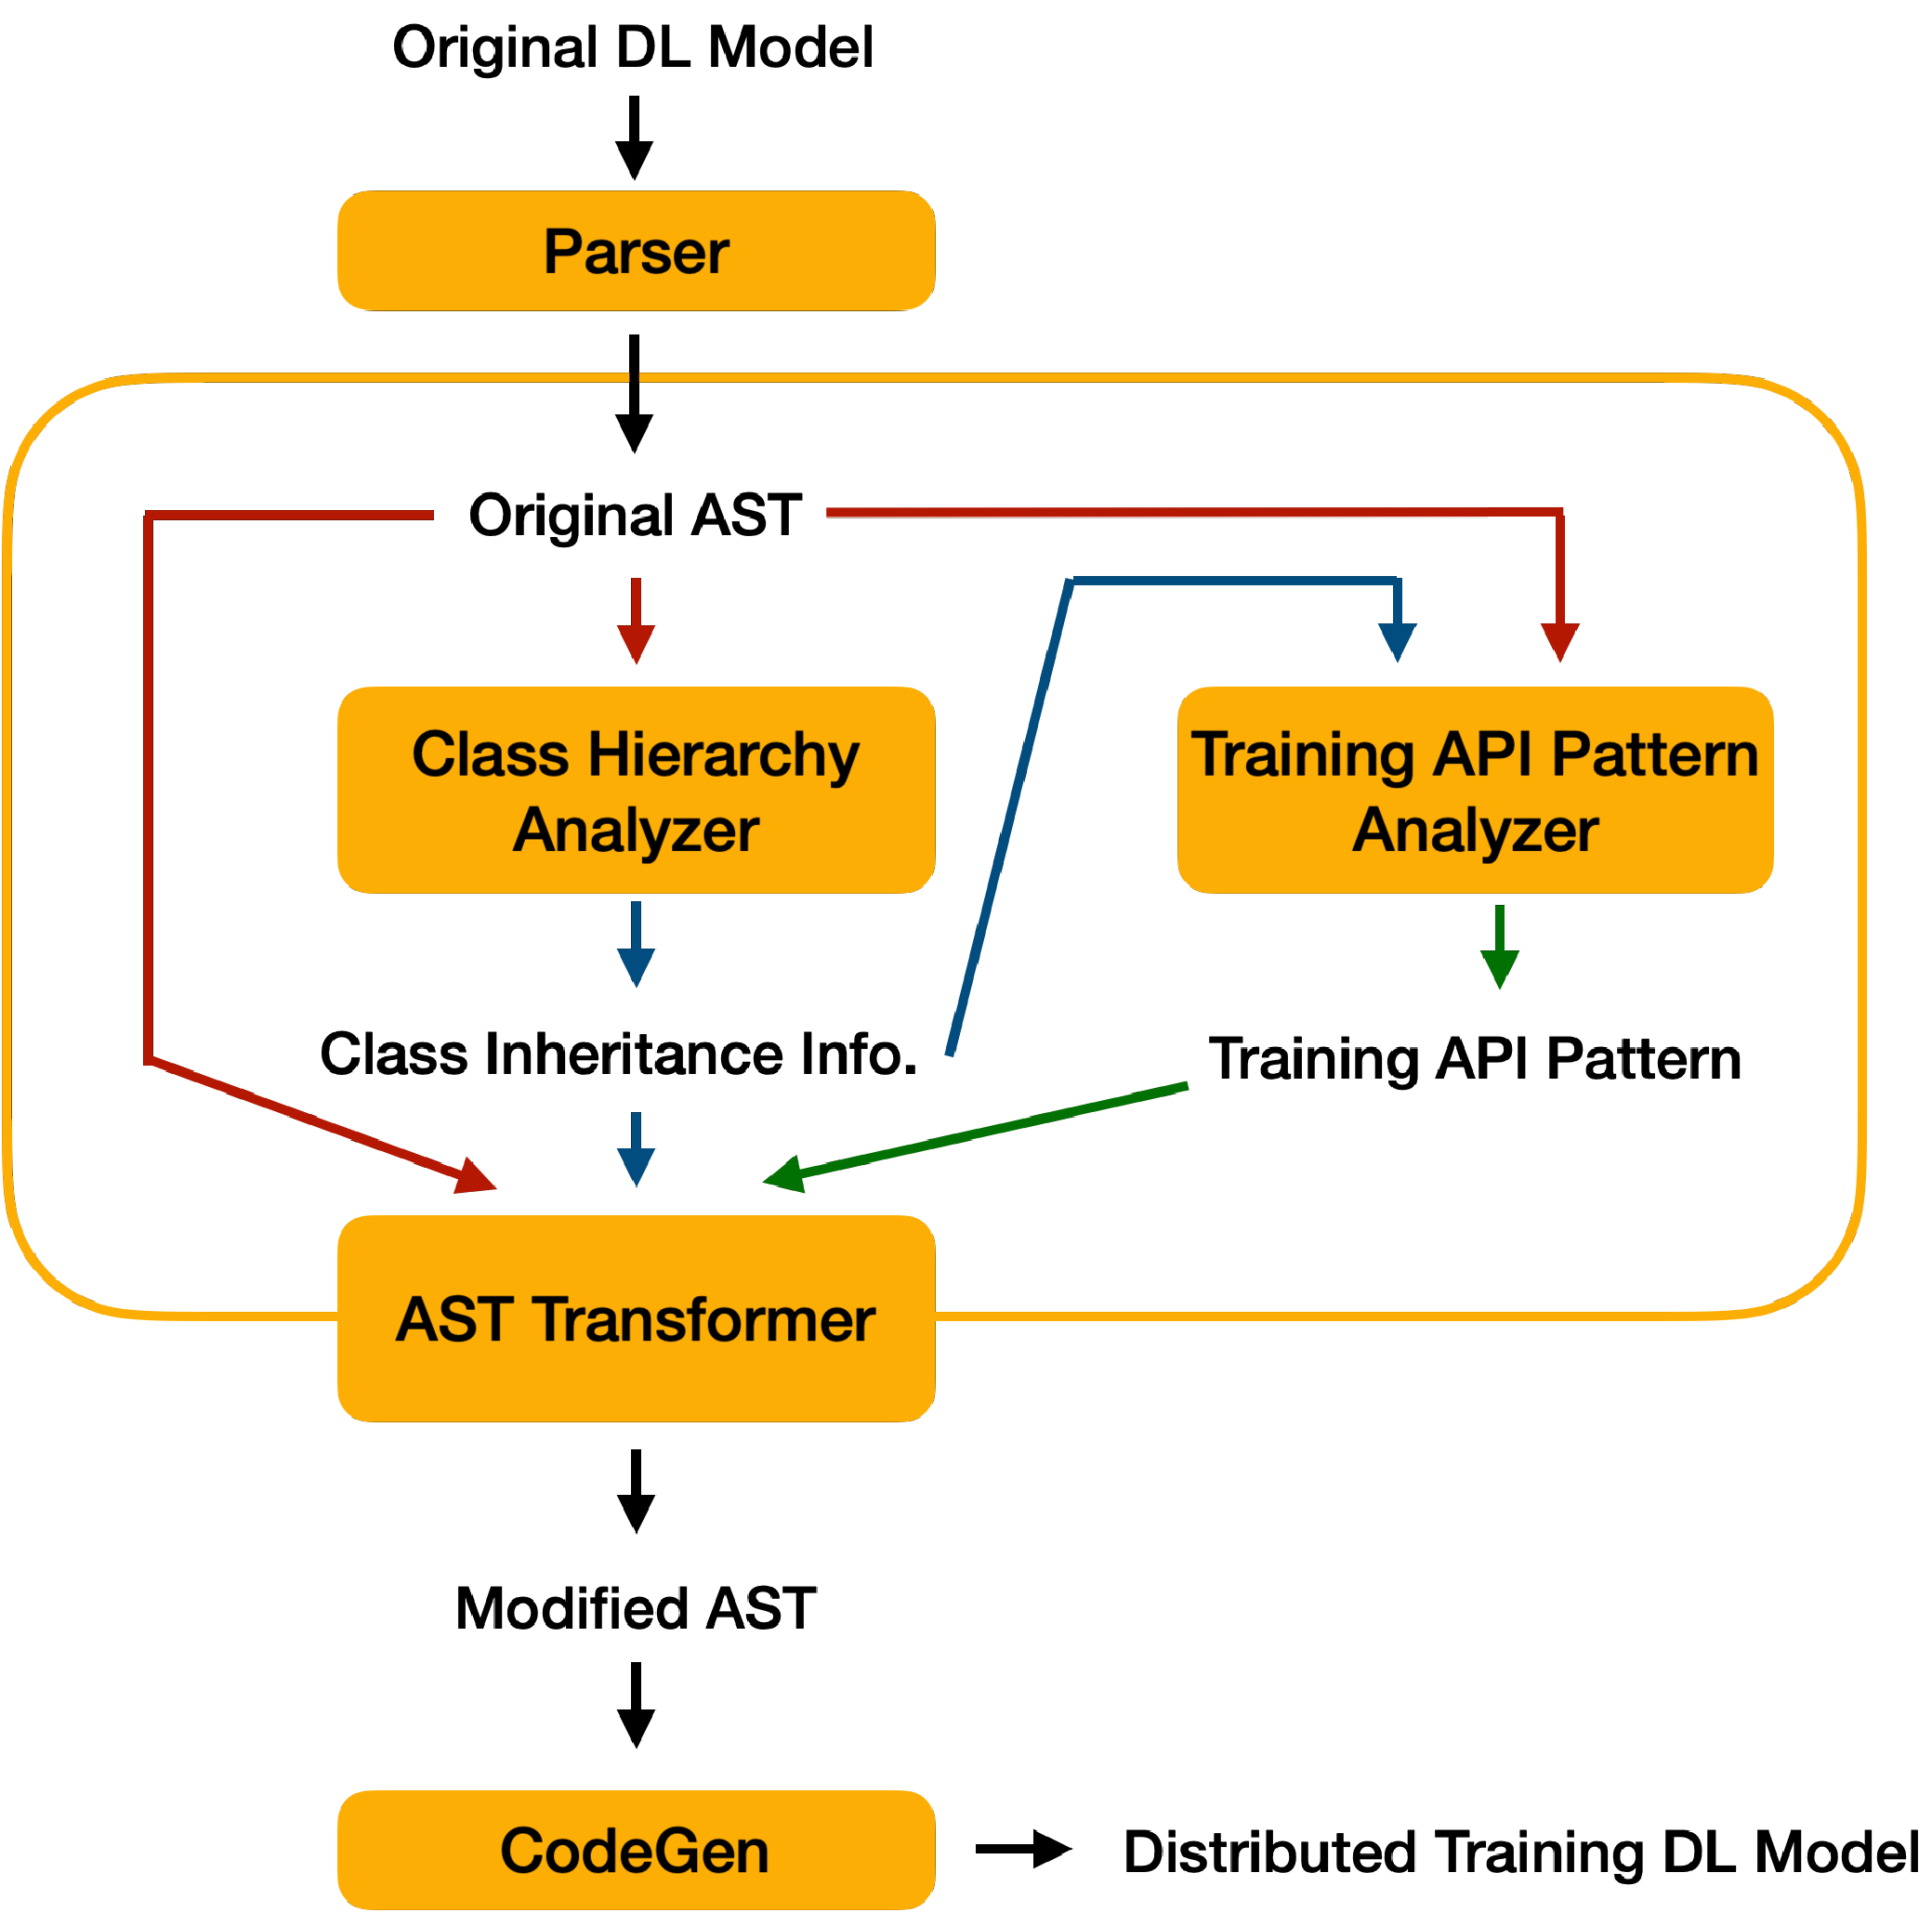
\includegraphics[width=0.5\textwidth]{tool-arch.pdf}
  \caption{The code transformation tool module design diagram}
  \label{sysarch}
\end{figure}

To correctly transform TensorFlow DL model, it is important to select
appropriate transformation rule for the type of the input training code.
This requires identifying the TensorFlow APIs appear in the code and
categorize them by their API patterns.
We devised to analyze \textit{class hierarchy} and \textit{API pattern} 
of the input training code and select appropriate transformation rule 
according to the analysis results. 

\textbf{Parser}
Parser is the module that parses input Python code package
into the set of ASTs.
We assume that the input single-GPU-based model is given as a Python code
package that resides in a single file directory.
Given the directory, the parser module first parses all Python code files
in the package to ASTs.
The Python abstract syntax and details on the parser implementation
are described in section \ref{sec:pysyn}.

Before the ASTs are transformed, the software performs two analyses, 
which are \textit{class hierarchy analysis} and 
\textit{API pattern analysis}.
These analyses provide necessary information to identify the
location and kind of the transformation target codes in the model
and select the correct transformation rule for the given input model.

\textbf{Class Hierarchy Analyzer}
Class hierarchy analyzer module analyzes the class inheritance relation
between user-defined classes and TensorFlow library classes and
outputs the class hierarchy graph.
During the API pattern analysis and AST transformation phase,
the software need to identify subclass relationship between
classes appearing in the code.
To support this, we implemented the class hierarchy analysis
for Python codes as the class hierarchy analyzer module.
The class hierarchy analyzer module produces the class hierarchy graph
for the model package and returns it to the API pattern analyzer and 
AST transformer modules. The details of the class hierarchy analyzer are
described in section \ref{sec:cha}.

\textbf{Training API Pattern Analyzer}
Training API pattern analyzer module 
indentifies the TensorFlow training APIs used in the training code AST
and returns the training API pattern for the code. (TODO: clarify?)
TensorFlow provides multiple APIs to define and invoke the training process.
To correctly transform a single-GPU-based model training code into
the distributed code, the transformation software must identify
training APIs used in the code and select the appropriate transformation rule.
The training API pattern analyzer matches the \textit{training API pattern}
against the input training codes to categorize them and select
the correct transformation rule. The details of the training API pattern
analyzer are described in section \ref{sec:pattern}.

\textbf{AST Transformer}
AST transformer module applies the correct transformation to the
training code AST to retain the distributed training code AST.
Here, the "correct" transformation is the set of transformation rules
appropriate for the given class hierarchy information and
training API pattern of the input training code.
We defined formal transformation rules which are composed of
\textit{transform functions} from ASTs to ASTs.
By applying the transform function to the input AST,
the AST transformer module outputs the transformed AST as an output.
The details of the AST transformer is described in section \ref{sec:trans}

%\section{Python Abstract Syntax and Parser}\label{sec:pysyn}
\subsection{Python Abstract Syntax}

We formalized the abstract syntax of the Python programming language.
For the reference, we refered to the full grammar specification in
Python Language Reference \cite{pythonref}. 
We manually examined the grammar specification 
to define the Python abstract syntax for our approach.
The figure \ref{fig:parse:abssyntax} illustrates the simplified
version of the Python abstract syntax we defined.
The Python languague is composed of three major components:
modules, statements, and expressions.

The top-level component of Python is a module, 
which is defined to be a statement.
In practce, Python modules contains series of statements;
this case is represented by statement sequence defined in our
Python abstract syntax.
In Python, multiple statements in the sequence are divided by newline. 

Statements are parts of the code that changes the program state.
For instance, assignment statement chanages the
value stored in the variable, and if-else statement changes
the control flow of the program.
In addition to the basic imperative statements,

Expressions are parts of the code that evaluates a value.
Python has composite types of a tuple, list, set, map, and custom classes.
The expression syntax defines ways to build up values
and complex expressions such as operators, comprehension, and function calls. 

\begin{figure}[!ht]
\begin{tabular}{lrll}
  \nmodule & := & \nstmt  \\
  \nstmt & ::= & \kdef ~ \nid ~ \sparen{\nargs} ~ \kcolon ~ \mul{\nstmt} & \desc{FunDef} \\ 
  & $|$ & \kclass ~ \nid ~ \sparen{\mul{\nexpr} \mul{\nkeyword}} ~ \kcolon ~ \mul{\nstmt} & \desc{ClassDef} \\
  & $|$ & \nexpr ~ \oassign \nexpr & \desc{Assign} \\
  & $|$ & \kfor ~ \nexpr ~ \kin ~ \nexpr ~ \kcolon ~ \mul{\nstmt} & \desc{ForLoop} \\
  & $|$ & \kwhile ~ \sparen{\nexpr} ~ \kcolon ~ \mul{\nstmt} & \desc{WhileLoop} \\
  & $|$ & \kif ~ \sparen{\nexpr} ~ \kcolon ~ \mul{\nstmt} ~ \op{(\kelse ~ \kcolon ~ \mul{\nstmt})}& \desc{If} \\
  & $|$ & \kwith ~ \mul{\nwithitem} ~ \kcolon ~ \mul{\nstmt} & \desc{With} \\
  & $|$ & \kimport ~ \mul{\nalias} & \desc{Import} \\
  & $|$ & \kfrom ~ \nint ~ \op{\nid} \kimport ~ \mul{\nalias} & \desc{ImportFrom} \\
  & $|$ & \nexpr & \desc{ExprStmt} \\
  & $|$ & \nstmt ~ {\tt \textbackslash n} ~ \nstmt  & \desc{Sequence} \\

  \nexpr & ::= & \nexpr ~ \nboolop ~ \nexpr & \desc{BoolOp} \\
  & $|$ & \nexpr ~ \nbinop ~ \nexpr & \desc{BinaryOp} \\ 
  & $|$ & \nunop ~ \nexpr & \desc{UnaryOp} \\ 
  & $|$ & \lparen{\mul{\nexpr}} & \desc{List} \\ 
  & $|$ & \sparen{\mul{\nexpr}} & \desc{Tuple} \\ 
  & $|$ & \nexpr ~ \sparen{\mul{\nexpr} \mul{\nkeyword}} & \desc{Call} \\
  & $|$ & \nconstant & \desc{Constant} \\
  & $|$ & \nexpr {\tt .}\nid& \desc{Attribute} \\
  & $|$ & \nid & \desc{Name} \\

  \nboolop & ::= & \oand ~ $|$ ~ \oor & \desc{BoolOperator} \\
  \nbinop & ::= & \oand ~ $|$ ~ \osub ~ $|$ ~ \omul & \desc{BinOperator} \\
  \nunop& ::= & \kinvert ~ $|$ ~ \knot ~ $|$ ~ \oadd ~ $|$ ~ \osub & \desc{UnOperator} \\
  \nargs & ::= & \mul{(\narg ~ \op{(\oassign ~ \nexpr)})}, ~ \mul{(\narg ~ \op{(\oassign ~ \nexpr)})}, ~ \op{\narg}, ~ \mul{(\narg ~ \op{(\oassign ~ \nexpr)})}, ~ \op{\narg} & \desc{Arguments}\\
  \narg & ::= & \nid ~ \op{\nexpr}~\op{\nstr} & \desc{Argument} \\
  \nkeyword & ::= & \op{\nid} \oassign \nexpr & \desc{Keyword} \\ 
  \nalias & ::= & \nid ~\mul{(.\nid)} \op{(\kas ~ \nid)} & \desc{Alias} \\
  \nwithitem & ::= & \nexpr ~ \op{(\kas ~ \nexpr)} & \desc{WithItem}\\

  \nconstant & ::= & \knone & \desc{NoneLiteral} \\
  & $|$ & \nint & \desc{IntLiteral} \\
  & $|$ & \nfloat & \desc{FloatLiteral} \\
  & $|$ & \nstr & \desc{StringLiteral} \\
  & $|$ & \nbool & \desc{BooleanLiteral} \\
  & $|$ & \sparen{\mul{\nconstant}} & \desc{TupleLiteral} \\
  \nid & $\in$ & \did \\
  \nstr & $\in$ & \dstr \\
  \nbool & $\in$ & \{{\tt True}, {\tt False}\}\\
  \nint & $\in$ & $\mathbb{Z}$ \\
  \nfloat & $\in$ & $\mathbb{R}$ \\
\end{tabular}
  \caption{Python abstract syntax}
  \label{fig:parse:abssyntax}
\end{figure}



\section{Class hierarchy analysis}\label{sec:cha}

When developing TensorFlow DL models, user-defined classes can
inherit TensorFlow library classes. 
This allows developers to extend the methods and behaviors of TensorFlow
library classes without directly modifying the library codes. 
Figure \ref{fig:cha:tfex}(a) shows an example of TensorFlow DL model
code using an user-defined class.
In line 4, the newly defined class {\tt ResNet} inherits the TensorFlow
library class, {\tt keras.Model}.
The {\tt keras.Model} class represents a model object composed of multiple
layers, and provides trainig-related methods such as {\tt compile} or {\tt fit}.
By inheriting the {\tt keras.Model} class, the {\tt ResNet} class
can also utilize the training-related methods while defining the new model
structure.
Line 8 creates a {\tt ResNet} class instance {\tt model}.
Then the line 9 calls the {\tt fit} method which is inherited from the
{\tt keras.Model} class.
By calling the {\tt fit} method, the model instance can be autoamtically
trained without manually repeating the training steps.

\begin{figure}[!ht]
  \centering
  \begin{subfigure}[t]{0.35\textwidth}
    \begin{lstlisting}[language=Python]
from tensorflow import keras

# `ResNet` inherits `keras.Model`
class ResNet(keras.Model): 
    def __init__(self, block_list):
        ...

model = ResNet([2,2,2])
model.fit(x_train, y_train)\end{lstlisting}
    \caption{Single-GPU-based DL model example using an user-defined class}
  \end{subfigure}
  \hspace{3mm}
  \begin{subfigure}[t]{0.6\textwidth}
    \begin{lstlisting}[language=Python]
from tensorflow import keras
import horovod.tensorflow.keras as hvd

class ResNet(keras.Model):
    def __init__(self, block_list):
        ...

model = ResNet([2,2,2])

model.fit(
    x_train, 
    y_train,
    callbacks=[hvd.callbacks.BroadcastGlobalVariablesCallback(0)])\end{lstlisting}
    \caption{Distributed model example using an user-defined class}
  \end{subfigure}

  \caption{Code example of distributing a model using an user-defined class}
  \label{fig:cha:tfex}
\end{figure}

To correctly transform TensorFlow DL models into the distributed models,
the transformation must recognize the user-defined classes that inherits
TensorFlwo classes.
Figure \ref{fig:cha:tfex}(b) is an example of modifying the code in 
\ref{fig:cha:tfex}(a) into a distributed model code.
Line 9 of \ref{fig:cha:tfex}(a) is modified as line 10 to 13 of 
\ref{fig:cha:tfex}(b). The modification adds a keyword argument {\tt callbacks}
to the {\tt fit} method call. 
To correctly modify the example code, the transformation must recognize the 
the line 9 of \ref{fig:cha:tfex}(a) calls the {\tt fit} method which originates
from the {\tt keras.Model} class.
Without recognizing the inheritance relation between {\tt ResNet} and
{\tt keras.Model}, the transformation module cannot correctly recognize
and modify the method call in line 9.  

To solve this problem, we employ the class hierarchy analysis as a pre-analysis
to analyze the class inheritance relation between user-defined classes
and TensorFlow classes.
\textit{Class hierarchy analysis} is a static analysis technique that identifies
inheritance relation between classes appear in the code.
By class hierarchy analysis on the input DL model code,
we can identify user-defined classes that inherit TensorFlow classes,
and therefore correctly identify training-related method calls.
In figure \ref{fig:cha:tfex}(a), for instance, 
the class herarchy analyzer reads line 4 to conclude that the user class
{\tt ResNet} is a subclass of {\tt keras.Model}.
The analysis result is sent to the later transformation stage,
which allows the transformation to recognize the {\tt fit} method
target in line 9 is inherited from the superclass, {\tt keras.Model}.

\pagebreak
\section{Training API Pattern Identification}\label{sec:pattern}

\subsection{Training API Patterns of TensorFlow DL Models}

\begin{figure}[ht!]
\centering
  \begin{subfigure}[b]{\textwidth}
    \begin{lstlisting}[language=Python]
for x, y in train_data.take(training_steps):
    with tf.GradientTape() as tape:
        pred = model(x, is_training=True)
        loss = loss_compute(y, pred)

    trainable_vars = model.trainable_variables
    gradients = tape.gradient(loss, trainable_vars)
    pairs = zip(gradients, trainable_vars)
    optimizer.apply_gradients(pairs) 
    \end{lstlisting}
    \caption{Using low-level training API}
  \end{subfigure}
  \hspace{5mm}
  \begin{subfigure}[b]{\textwidth}
    \begin{lstlisting}[language=Python]
model.compile(
    optimizer = optimizer, 
    loss = loss_compute) 
model.fit(train_data.take(training_steps))
    \end{lstlisting} 
    \caption{Using high-level training API}
  \end{subfigure}

  \caption{TensorFlow model code example using two different API patterns}
  \label{fig:pattern:ex01}
\end{figure}

% tf 모델을 바르게 변환하기 위해서는,  서로 다른 훈련 api를 사용하느 ㄴ모델을
% 분류하고, 각 분류의 모델에 다른 변환을 적용할 필요가 있다.
In TensorFlow models, developers can use different APIs to define the 
model structure and training process.
The figure \ref{fig:pattern:ex01} illustrates two TensorFlow model codes that
use different APIs to define the training process.
The lines 2 to 10 in \ref{fig:pattern:ex01}(a)  
explicitly repeats the training steps by using the {\tt for} loop
and the {\tt GradientTape} instance.
In contrast, the lines 1 and 4 in \ref{fig:pattern:ex01}(b)
use the Keras library API {\tt fit} to invoke the training process.
While both codes train the model in the same way, they use different training 
APIs in different patterns.
As their API usages are significantly different, our transformation approach
need to apply different transformation rules.

\begin{figure}[ht!]
  \centering
  \begin{tabular}{|c|c|l|}
    \hline
    TF version & Pattern name & Explanation \\
    \hline
    1.x & Session & 
	  The models using the {\tt Session} API to invoke training operations\\
    \hline
    1.x & MonitoredSession & 
	  The models using the {\tt MonitoresSession} API to invoke 
	  training operations.\\
    \hline
    2.x & GradientTape & 
	  The models using the {\tt GradientTape} API to explicitly 
	  repeat the training step.\\
    \hline
    2.x & Keras & 
	  The models using {\tt keras.Model} class to define the model
	  and the {\tt fit} API to train the model.\\
    \hline
  \end{tabular}
  \caption{Training API patterns}
  \label{tab:patterns}
\end{figure}

% 서로 다은 훈련 api를 사용하는 모델을 분류하기 위해서 우리는 4개의
% training api pattern을 정의햇다.
To categorize the TensorFlow DL models by their training API usage,
we manually inspected open-source TensorFlow models and
defined four \textit{training API patterns} that categorizes them.
The training API patterns are the code patterns of TensorFlow APIs 
that commonly appear in the same categories of the models.
For instance, the models in the same category with the figure
\ref{fig:pattern:ex01}(a) use the {\tt with} statements that create the
{\tt GradientTape} objects.
We patternize such common API usages into the training API patterns and
utilize to categorize the TensorFlow DL models.
Figure \ref{tab:patterns} describe the four training API patterns defined
for TensorFlow DL models.
The following paragraphs explain the details of each training API pattern.



% 우리가 정의한 4가지의 api pattern은 피규어의 표와 같다. 
% Figure \ref{tab:patterns} describes the four training API patterns.
% The Session pattern and the MonitoredSession pattern categorizes the
% TensorFlow 1.x models. The GradientTape pattern and the Keras pattern
% categorizes the TensorFlow 2.x models.
% Based on the training API patterns,
% we implement the \textit{training API pattern identifier} to
% categorize the input model.
% The training API pattern identifier matches each training API pattern
% against the input model codes. 
% If the code successfully matches in exactly one pattern,
% the training API pattern identifier categorizes the input model into
% the corresponding pattern.
% If the code fails to match a pattern or is matched into more than one patterns,
% the training API pattern identifier raises exception that the input model
% cannot be automatically transformed by our approach.


\subsubsection{Session Pattern}

\begin{figure}[!ht]
\begin{lstlisting}[language=Python]
with tf.Session() as sess:
    for images, labels in dataset.take(10000):
        sess.run(train_op, {x: images, y: labels})
\end{lstlisting}
\caption{Session pattern code example}
\label{fig:sessionpattern}
\end{figure}

The Session pattern categorizes the TensorFlow 1.x models that
use the {\tt Session} class instance to manually invoke the training 
computation. Figure \ref{fig:sessionpattern} is a code example of the Session 
pattern. In line 1, the {\tt with} statment creates the {\tt Session}
class instance. In the line 3, the {\tt run} method is called to invoke 
the training computation. 
In the {\tt with} statement body, the {\tt run} method can be called multiple
time to invoke computation of arbitrary TensorFlow operations.
In practice, developers use {\tt while} or {\tt for} loops to repeatedly call
the {\tt run} methods to trigger the training step on multiple training batches,
as the line 2 in the figure \ref{fig:sessionpattern}.

To identify the Session pattern model, the identifier 
searches for a {\tt with} statement that creates the {\tt Session} instance.
If the body statements of the {\tt with} statement call the 
{\tt run} method of the {\tt Session} instance,
the identifier categorizes the input model as the Session pattern. 


\subsubsection{MonitoredSession Pattern}

\begin{figure}[!ht]
  \begin{lstlisting}[language=Python]
summary_hook = SummarySaverHook(...)

with MonitoredTrainingSession(hooks=[summary_hook]) as mon_sess:
    while not mon_sess.should_stop():
        mon_sess.run(train_op, feed_dict=feed_dict)
  \end{lstlisting}
  \caption{MonitoredSession pattern code example}
  \label{fig:monsesspattern}
\end{figure}

The MonitoredSession pattern categorizes TensorFlow 1.x models that
use the {\tt MonitoredSession} class instance to manually invoke the 
training computation.
Figure \ref{fig:monsesspattern} is a code example of the MonitoredSession 
pattern.
In the line 3, the {\tt with} statement creates the {\tt MonitoredSession}
class instance with the {\tt MonitoredTrainingSession} API.
The line 5 calls the {\tt run} method of the {\tt MonitoredSession} instance 
to invoke the training computation.
Developers can add the \textit{hooks} to the
{\tt MonitoredSession} instance. The hooks are actions that automatically 
executed upon specific conditions. 
For instance, the line 3 adds the {\tt SummarySaverHook} to the
{\tt MonitoredSession}, a hook which automatcially saves the model summary 
after every {\tt run} method call.

To identify the MonitoredSession pattern training code,
the identifier searches for a {\tt with} statement that creates a
{\tt MonitoredSession} instance by {\tt MonitoredTrainingSession} API.
If the body statements of the {\tt with} statement call the {\tt run} methods 
of the {\tt MonitoredSession} instance, 
the identifier categorizes the input model as the MonitoredSession pattern. 


\subsubsection{GradientTape Pattern}

\begin{figure}[!ht]
  \begin{lstlisting}[language=Python]
optim = tf.optimizers.Adam(0.001)

for images, labels in dataset.take(10000):
    with tf.GradientTape() as tape:
        probs = model(images)
        loss_value = loss(labels, probs)

    grads = tape.gradient(loss_value, model.trainable_variables)
    optim.apply_gradients(zip(grads, model.trainable_variables))
  \end{lstlisting}
  \caption{GradientTape pattern code example}
  \label{fig:tapepattern}
\end{figure}


The GradientTape pattern categorizes TensorFlow 2.x models that
use the {\tt GradientTape} class instance to manually invoke training 
computations. Figure \ref{fig:tapepattern} is a code example of 
GradientTape pattern.
In line 3, the {\tt with} statement creates the {\tt GradientTape} class
instance. 
After the {\tt with} statement, the line 8 calls the {\tt gradient} method
to retreive the recorded gradients of the model.
The line 9 calls the {\tt apply\_gradients} methods of the {\tt Optimizer}
class instance to finally update the model parameters.

To identify a GradientTape pattern model,
the identifier searches for the {\tt with} statement that creates a
{\tt GradientTape} instance.
The identifier also searches for the {\tt Optimizer} instance 
{\tt apply\_gradients} method call.
If identifier finds both of the statements, the identifer categorizes the
model as the GradientTape pattern.


\subsubsection{Keras Pattern}

\begin{figure}[ht!]
  \begin{lstlisting}[language=Python]
class ResNet(keras.Model):
    def __init__(self, params):
        ...

model = ResNet([2, 2, 2], num_classes)
model.fit(dataset, epochs=50)\end{lstlisting}
 
  \caption{Keras pattern code example}
  \label{fig:keraspattern}
\end{figure}

The Keras pattern categorizes TensorFlow 2.x models that use
the {\tt keras.Model} class method {\tt fit} to train the model. 
Figure \ref{fig:keraspattern} is a code example of Keras pattern.
The line 1 defines the {\tt ResNet} class that inherits the 
{\tt keras.Model} class. 
The line 5 creates the {\tt ResNet} class instance.
The line 6 calls the {\tt fit} method to train the model.
Note that the {\tt fit} method is inherited from the {\tt keras.Model} class.

To identify a Keras pattern model, the identifer searches for the
{\tt Model.fit} method call. The training API pattern identifier utilizes the
class inheritance information provides by the class hierarchy analyzer to
recognize subclasses of the {\tt keras.Model} class and their instances.
If identifier find the {\tt fit} method call of the {\tt keras.Model} subclass
instance, the identifier categorizes the model as the Keras pattern.

\subsection{Training API Pattern Identifier}

We implemented the training API pattern identifier, which classifies the
input TensorFlow model into one of the four patterns.
The training API pattern identifier scans through the input model AST,
detects statements that match one of the four traning API patterns.
One caveat here is that the input model can no statements or multiple statements
that match the training API patterns.
In these cases, the identifier must notify user that the
input model is not available for automatic transformation.
To implement this, we define a flat lattice structure composed of four 
training API patterns and the top and bottom elements.
The lattice structure is described in figure \ref{fig:pattern:lattice}.
The training api pattern identifier returns one of the six elements of
the lattice. The bottom element means that the input model does not have
statements that matches with the training API patterns.
The top elements means that the input model has statements that matches with
more than one of the training API patterns.
In both cases, the input model is not available for the automatic 
transformation, resulting in abortion of the tranformation process.

\begin{figure}[ht!]
  \centering
  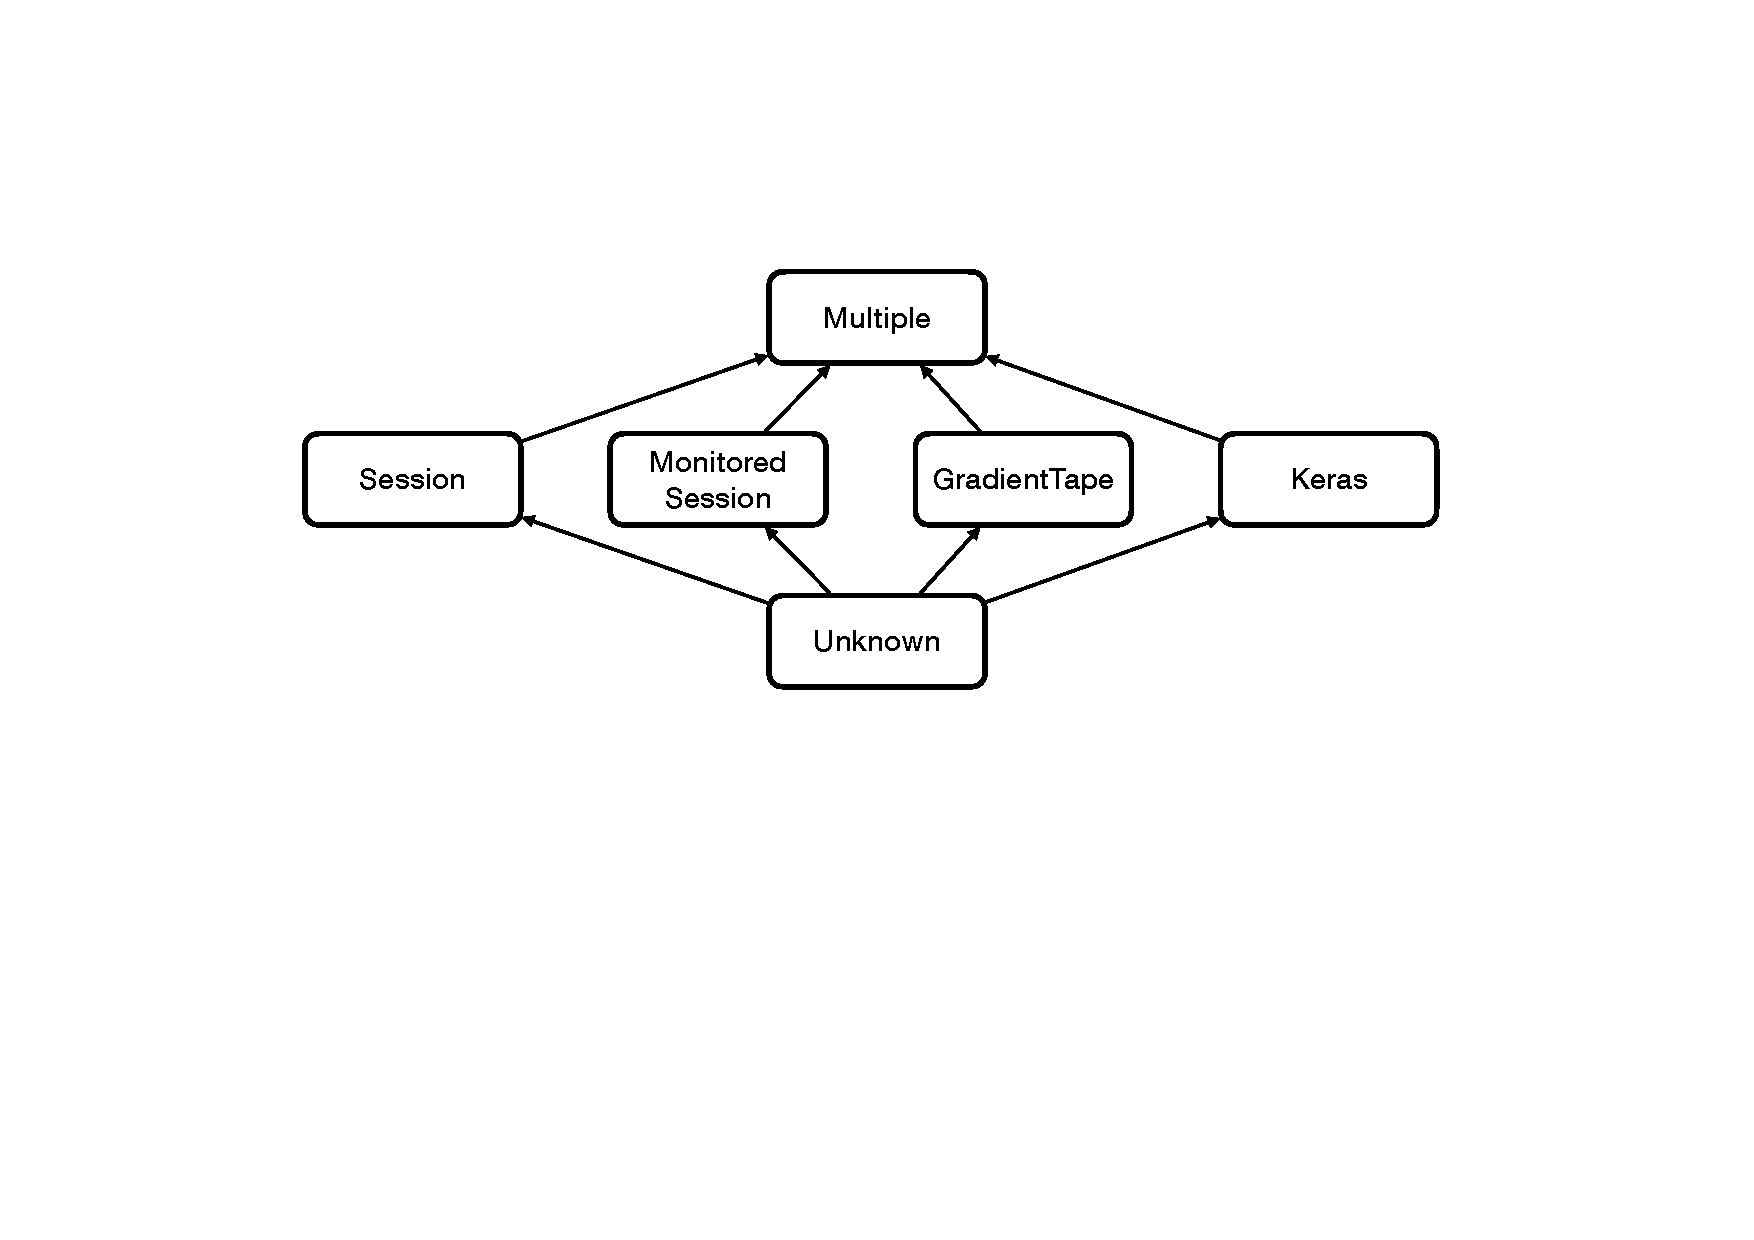
\includegraphics[width=0.7\textwidth]{lattice.pdf}
  \caption{The flat lattice structure of four traininig API patterns}
  \label{fig:pattern:lattice}
\end{figure}


% TODO put algorithm blocks inside the figure env.
% algo related macro
\algblockdefx{Match}{EndMatch}{\textbf{Match}}{}
\algblockdefx{Case}{EndCase}{\textbf{case}}{}
\algtext*{EndMatch}
\algtext*{EndCase}

\algblockdefx{Enum}{EndEnum}{\textbf{Enum}}{}
\algtext*{EndEnum}

% lattice
% \begin{algorithm}[ht!]
%   \caption{Training API pattern lattice}
%   \begin{algorithmic}[1]
%     \Enum~Pattern
%     \State Top
%     \State SessionPattern 
%     \State MonitoredSessionPattern
%     \State GradientTapePattern
%     \State KerasPattern
%     \State Bot
%     \EndEnum
%     
%     \Function{Union}{$x$, $y$} \Comment{Union of two Patterns, x $\cup$ y}
%     \Match~($x$, $y$)~\textbf{with:}
%       \Case~(Bot, $p$) | ($p$, Bot): $p$ \EndCase
%       \Case~\_: Top \EndCase
% 
%     \EndMatch 
%     \EndFunction
%   \end{algorithmic}
%   \label{fig:pattern:algo1}
% \end{algorithm}

% pseudocode
\begin{algorithm}
\caption{Training API pattern identifier}\label{tapa}
  \begin{algorithmic}[1]
    \Function{IdentifyPattern}{$AST$}
    \Match~$AST$~\textbf{with:}

      \Case~{\tt with Session() as}~$name$~{\tt :}~$body$
        \If{$body$~includes~$name${\tt.run()}}
          SessionPattern
        \EndIf
      \EndCase

      \Case~{\tt with MonitoredTrainingSession() as}~$name$~{\tt :}~$body$
        \If{$body$~includes~$name${\tt.run()}}
          MonitoredSessionPattern
        \EndIf
      \EndCase

      \Case~{\tt with GradientTape() as}~$name$~{\tt :}~$body$
        \If{$AST$.parent~includes~$name${\tt.apply\_gradients()}}
          GradientTapePattern
        \EndIf
      \EndCase

      \Case~$model${\tt.fit(...)}
        \If{$model$.class~isSubclassOf~{\tt keras.Model}}
          KerasPattern
        \EndIf
      \EndCase

      \Case~\_
        \If{$AST$.isSimpleStatement}
          Bot 
        \Else
          \State \textbf{Let} childrenPatterns \textbf{=} $AST$.childrenStatements.map(s => IdentifyPattern(s))
          \State childrenPatterns.fold((p1, p2) => p1 $\cup$ p2) 
        \EndIf
      \EndCase

    \EndMatch
    \EndFunction
  \end{algorithmic}
\end{algorithm}

Figure \ref{???} is the pseudocode of the training API pattern identifier.
The function {\tt IdentifyPattern} gets and input AST and returns a training
API pattern lattice element.
The algorithm first matches the statement with four training API patterns.
Lines 3 and 4 match if the input AST is a {\tt with} statement that
creates a {\tt Session} instance and call the {\tt run} method in the body.
If the match succeeds, the algorithm returns Session pattern.
Lines 5 and 6 match if the input AST is a {\tt with} statement that
creates a {\tt MonitoredSession} instance and call the {\tt run} method in the
body.
If the match succeeds, the algorithm returns MonitoredSession pattern.
Line 7 matches if the input AST is a {\tt with} statement that
creates a {\tt GradientTape} instance.
Line 8 then matches if the parent AST has a child statement that calls the
{\tt apply\_gradients} method of the {\tt GradientTape} instance.
If both matches succeed, the algorithm returns GradientTape pattern.
Line 9 and 10 matches if the input AST is a statement that calls
the {\tt fit} method of a subclass of {\tt keras.Model}. 
If the match succeeds, the algorithm returns Keras pattern.

Lines 11 to 15 describe the cases where the input AST does not match with 
one of the four training API patterns.
If the input AST is a simple statement, which does not have child ASTs,
the algorithm returns the bottom element.
Else, the algorithm recursively identifies the pattern of the child ASTs
then return the join of the results.
If the child ASTs are matched with multiple training API patterns, 
the algorithm will return the top element.

\pagebreak

\section{Code Transformation}\label{sec:trans}
\subsection{Transformation Rule for Distributed TensorFlow ML model}

In this section, we describe the transformation rule that
transforms single-GPU-based TensorFlow model codes into
multi-GPU-based TensorFlow model codes.
We informally understand code transformation rule as
conditions to select the target code parts
and methods to transform them into another.
The methods include the addition, modification, and deletion of
specific code parts.
Currently, code transformation for distributed ML training
is only described by a set of examples and informal explanations.
To automate the code transformation process,
we need to formally define the code transformation rule
and ways to convert the definition into software implementation.
We propose a formal definition of the code transformation rule
for distributed ML training and implement the automatic code transformation
software based on the formal definition.

Code transformation is formally defined as a pure function from AST to AST.
We call this function a transform function.
We may define multiple transform functions that act on different
language constructs and use them to define other transform functions.
For example, to transform a Python code into another,
we define a transform function that takes Module AST and returns Module AST.
Inside the Module transform function definition,
we may use the statement transform function to transform statements
that compose the Module AST.

Together with the AST parameter, transform functions take and return
the environment parameter.
Environment parameters are used to store specific identifiers
and pass them to the other calls of the transform function.
For example, the statement transform function frequently uses 
the identifier bound to the TensorFlow module.
The module name first appears from the import statement.
The transform function call on the import statement stores
the TensorFlow module name on the environment and returns it.
Then the later function calls to other statements
retrieve the TensorFlow module name from the environment parameter.

% explain transform function with example

\begin{figure}[h]
\begin{lstlisting}[language=Python]
import tensorflow as tf
optimizer = tf.keras.optimizers.Adam(lr)
\end{lstlisting}
  \caption{Original code example}
  \label{fig:trans:org}
\end{figure}

\begin{figure}[h]
\begin{lstlisting}[language=Python]
import tensorflow as tf
# import and init horovod module
import horovod.tensorflow as hvd
hvd_broadcast_done = False
hvd.init()
import tensorflow.keras as keras

# scale the learning rate
optimizer = tf.keras.optimizers.Adam(lr * hvd.size())
# wrap the optimizer object
optimizer = hvd.DistributedOptimizer(optimizer)
\end{lstlisting}
  \caption{Transformed code example}
  \label{fig:trans:hvd}
\end{figure}

We first describe how the transform function works by example.
The above figures illustrate a pair of TensorFlow model codes
before and after the transformation;
the figure \ref{fig:trans:org} represents the original
training code before the transformation and
the figure \ref{fig:trans:org} represents the distributed
training code after the transformatioin.
Informally, three kinds of transformation occur in between;
1) import and initialize the horovod module;
2) scale the optimizer's learning rate by {\tt hvd.size()};
3) Wrap the optimizer with {\tt hvd.DistributedOptimizer}.

The original code parses into a module AST with a list of 2 statements,
an import statement and an assign statement, 
as illustrated in the figure \ref{fig:trans:ast}. 

\begin{figure}[h]
\begin{lstlisting}[language=Scala]
Module(List(
  ImportStmt(Id('tensorflow'), Id('tf')),
  AssignStmt(
    Id('optimizer'), 
    CallExpr(
      Expr('tf.keras.optimizers.Adam'),
      Args(Id('lr'))
    )
  )
))
\end{lstlisting}
  \caption{The AST of the code in figure \ref{fig:trans:org}, represented in Scala object}
  \label{fig:trans:ast}
\end{figure}

\begin{figure}[!ht]
\begin{tabular}{lcl}
  \tmodule{[\nstmtsubs{1}, \nstmtsubs{2}] ~ \ntypignore} 
  & \kteq & \tsstmt{[\nstmtsubs{1}, \nstmtsubs{2}]}{\smodenvempty} \\

  & \kteq & \ktlet ~ \mul{\nstmtsubs{1}}$'$, \smodenvsubs{1} ~ \kteq ~ 
  \tstmt{\nstmtsubs{1}}{\smodenvempty} ~ \ktin \\

  & & \ktlet ~ \mul{\nstmtsubs{2}}$'$, \smodenvsubs{2} ~ \kteq ~ 
  \tstmt{\nstmtsubs{2}}{\smodenvsubs{1}} ~ \ktin \\

  & & (\mul{\nstmtsubs{1}}$'$ \ktconl ~ \mul{\nstmtsubs{2}}$'$) \\ 
\end{tabular}
  \caption{Transform function evaluated on the module AST}
  \label{fig:trans:ex_module}
\end{figure}

The figure \ref{fig:trans:ex_module} 
describes how the module transform function 
is evaluated on the example module AST.
The module transform function, $\fkmodule$
applies statement list transform function $\fksstmt$ to its statement list.
Then $\fksstmt$ applies the statement transform function $\fkstmt$
to each statement in the list.
In addition, $\fksstmt$ passes the environment parameter $\sigma$
from a $\fkstmt$ call to the next $\fkstmt$ call.

The figure \ref{fig:trans:ex_stmt1} illustrates the evaluation of
the transform function on \nstmtsubs{1}.
The first $\fkstmt$ call receives the statement
{\tt import tensorflow as tf} as an input.
In part (a), the function first matches the input statement
with the pattern $\kimport ~ \mul{\nalias}$.
Transform functions use pattern matching to discriminate target ASTs
by their syntactic structure.
Part (b) specifies the pattern guard, which describes the detailed conditions
on the content of the input.
The pattern guard checks if the import statement
is importing the TensorFlow module.
In the process, the alias transform function $\fkalias$ is applied on the
{\tt tensorflow as tf}.
Note that $\fkalias$ also stores the module name {\tt tf}
in the environment parameter as a form of mapping;
later calls on the transform function can retrieve the
TensorFlow module name from the returned environment, $\smodenvsubs{1}$.
Finally, part (c) constructs the output statements
and returns it with $\smodenvsubs{1}$.


\begin{figure}[!ht]
\begin{tabular}{rcll}
  \tstmt{\nstmtsubs{1}}{\smodenvempty} & \kteq & 
  \tstmt{{\tt import tensorflow as tf}}{\smodenvempty} & \\

  & \kteq & \tstmt{\kimport ~ \mul{\nalias}}{\smodenvempty} & 
  (a) Pattern matching the input \\

  & & {\tt matching} ~ ( & \\
  && \indent \kimport ~ \mul{\nalias} \kteq ~ 
  \kimport ~ [{\tt tensorflow} \kas ~ {\tt tf}], & \\
  && \indent \mul{\nalias} \kteq ~ [\naliassubs{1}], & \\ 
  && \indent \naliassubs{1} \kteq ~ {\tt tensorflow} \kas ~ {\tt tf} ~ ) & \\

  & \kteq & 
  \ktlet ~ \smodenvsubs{1} ~ \kteq ~ \taalias{[\naliassubs{1}]}{\smodenv} 
  \ktin & 
  (b) Check if the TensorFlow module imported \\
  && \ktif ~ \smodenvsubs{1} ~ \envsub ~ \smodenv ~ 
  \kteq ~ [\tflow $\mapsto$ \nid] ~ \ktthen &\\ 
  && ([\kimport ~ \naliassubs{1}, & \\
  && {\tt import horovod.tensorflow as hvd}, & \\
  && {\tt hvd\_broadcast\_done = False}, & \\
  && {\tt hvd.init()}], \smodenvsubs{1}) & \\
  
  & \kteq &
  ([\kimport ~ {\tt tensorflow} \kas ~ {\tt tf}, & 
  (c) Construct output statements \\
  && {\tt import horovod.tensorflow as hvd}, & \\
  && {\tt hvd\_broadcast\_done = False}, & \\
  && {\tt hvd.init()}], \smodenvsubs{1}) & \\

  \kwith ~ \smodenvsubs{1} 
  & \kteq & \talias{\naliassubs{1}}{\smodenvempty} & \\
  & = & \talias{{\tt tensorflow} \kas ~ {\tt tf}}{\smodenvempty} & \\ 
  & \kteq & \smodenvempty[\tflow $\mapsto$ {\tt tf}] & \\
  & \kteq & [\tflow $\mapsto$ {\tt tf}] & \\
\end{tabular}
  \caption{Transform function evaluated on the first statement AST}
  \label{fig:trans:ex_stmt1}
\end{figure}

\begin{figure}
\begin{tabular}{rcll}
  \tstmt{\nstmtsubs{2}}{\smodenvempty} & \kteq &
  \tstmt{{\tt optimizer = tf.keras.optimizers.Adam(lr)}}{\smodenvsubs{1}} &\\
  &\kteq&
  \tstmt{\nidsubs{r} \oassign 
  \nexprsubs{1} \sparen{\nexprsubs{11} ... \nexprsubs{1n} ~ 
  \op{(\nidsubs{1} \oassign)} \nexprsubs{21} ... 
  \op{(\nidsubs{k} \oassign)} \nexprsubs{2k}}}{\smodenvsubs{1}} &\\
  && {\tt matching} ~ ( 
  \indent\indent\indent\indent\indent (a) Pattern matching the input &\\
  && \indent \nidsubs{r} \kteq ~ {\tt optimizer}, &\\
  && \indent \nexprsubs{1} = {\tt tf.keras.optimizers.Adam}, &\\
  && \indent \nexprsubs{11}= {\tt lr}~) &\\

  &\kteq& \ktif ~ \smodenvsubs{1}(\tflow) ~ \kteq ~ \nidsubs{t} ~ 
  \indent\indent\indent\indent\indent
  (b) Check if it calls {\tt tf.keras.optimizers.Adam} &\\ 
  && \ktand ~ 
  \nexprsubs{1} ~ \kteq ~ {\tt \nidsubs{t}.keras.optimizers.Adam} ~ 
  \ktthen& \\

  && ([\nidsubs{r} \oassign \nexprsubs{1} 
  \sparen{\nexprsubs{11} {\tt * hvd.size()} ~ ... ~ \nexprsubs{1n} 
  ~\op{(\nidsubs{1} \oassign)} \nexprsubs{21} ... 
  \op{(\nidsubs{k} \oassign)} \nexprsubs{2k}}], &\\
  && \smodenvsubs{1}[\optmizer $\mapsto$ \nidsubs{r}])&\\
  
  &\kteq& 
  ([{\tt optimizer = tf.keras.optimizers.Adam(lr * hvd.size())}], &\\   
  && \smodenvsubs{1}[\optmizer $\mapsto$ \nidsubs{r}])
  \indent\indent\indent\indent\indent
  (c) Construct output statements &\\ 
\end{tabular}
  \caption{Transform function evaluated on the second statement AST}
  \label{fig:trans:ex_stmt2}
\end{figure}

The figure \ref{fig:trans:ex_stmt2} illustrates the evaluation of
the transform funcion on \nstmtsubs{2}.
The second $\fkstmt$ receives the statement
{\tt optimizer = tf.keras.optimizers.Adam(lr)} as an input.
Part (a) pattern matches the input to the assign statement pattern
with the right-hand side of the function call expression.
Part (b) is a pattern guard that checks if
the function call is {\tt tf.keras.optimizers.Adam}.
Note that the guard refers to the environment parameter
to check the TensorFlow module identifier.
Because after the first $\fkstmt$ call,
the environment parameter stores the TensorFlow module identifier {\tt tf},
so the second $\fkstmt$ call can use the information to
check if the function call is indeed a constructor for TensorFlow
optimizer object.
In part (c), the output statement is returned.
As specified in the transform function definition, 
the first argument expression is multiplied by {\tt hvd.size()}.

\begin{figure}[!ht]
\begin{tabular}{rcll}
  \tmodule{[\nstmtsubs{1}, \nstmtsubs{2}] ~ \ntypignore} 
  &\kteq& (\mul{\nstmtsubs{1}}$'$ \ktconl ~ \mul{\nstmtsubs{2}}$'$) &\\ 
  &\kteq& 
  [\kimport ~ {\tt tensorflow} \kas ~ {\tt tf}, &\\ 
  && {\tt import horovod.tensorflow as hvd}, & \\
  && {\tt hvd\_broadcast\_done = False}, & \\
  && {\tt hvd.init()}, &\\
  && {\tt optimizer = tf.keras.optimizers.Adam(lr * hvd.size())}] &\\   
\end{tabular}
  \caption{Transform function concatenating the resulting statements}
  \label{fig:trans:ex_concat}
\end{figure}

Finally, the output statement lists are concatenated as specified in the
$\fksstmt$, and the transformed module AST is constructed
as illustrated on the figure \ref{fig:trans:ex_concat}.

As described in the example, the transform functions are defined for
each language construct. The functions are described in terms of
pattern matching against the input AST; the matching patterns and 
pattern guards select the target AST to transform, and
the output AST is constructed with the matched variables.

Each training API category defines a corresponding transform function.
Given a training code of the category, the corresponding module AST transform
function is applied to the target code AST with an empty environment parameter.
In the following subsections, we describe the transform function for each
training API category. The paper only explains important parts of the 
definition; the full definition of the transform functions can be found
in the supplementary material.

\subsection{Description of Transform functions}

\subsubsection{Transform function for Session pattern}

The training codes in Session pattern and MonitoredSesion pattern
use legacy version of the TensorFlow 1.x library. 
These legacy codes can be identified by specific import statement as below.

\begin{figure}[h]
\begin{lstlisting}[language=Python]
import tensorflow.compat.v1 as tf
\end{lstlisting}
\caption{Import statements for using TensorFlow 1.x legacy module}
\end{figure}

Session pattern and MonitoredSesison pattern uses the following
transform function to match the legacy import statement
and add the import statement for Horovod library.

\begin{figure}[h]
\noindent
\begin{longtable}{l}
  \tstmt{\kimport ~ \mul{\nalias}}{\smodenv} = \\
  \inden \ktif ~ \smodenvsubs{1} ~ \envsub ~ \smodenv ~ \kteq ~ [\tflowc $\mapsto$ \nid] ~ \ktthen \\
  \inden\hspace{1em} ([\kimport ~ \mul{\nalias}, \\
  \inden\hspace{1em} \kimport ~ {\tt horovod.tensorflow} \kas ~ {\tt hvd}, \\
  \inden\hspace{1em} {\tt hvd.init()}], \smodenvsubs{1})\\
  \inden \ktelse~([\kimport ~ \mul{\nalias}], \smodenvsubs{1})
\end{longtable}
\caption{Session pattern transform function: Importing Horovod}
\end{figure}

The Session pattern codes use the {\tt Session} object to define the computation environment.
The {\tt Session} objects are usually defined by {\tt With} statements,
and later used by calling the method {\tt Session.run}.
(TODO: add explanation)

The {\tt Optimizer} instances must be modified for distributed training.
First, the learning rate is scaled by {\tt hvd.size()},
and the optimizer instance is wrapped with {\tt hvd.DistributedOptimizer}.
The following rule describes the part of the transform function that
performs learning rate scaling and the wrapping.
The function matches an assignment statement that assigns an
instance of {\tt Optimizer} class, and modifies the learning rate argument
given the the instance constructor. Then the rule appends the statement
that wraps the {\tt Optimizer} instance with {\tt hvd.DistributedOptimizer}.

\begin{figure}[h]
\noindent
\begin{longtable}{l}
  \tstmt{\nidsubs{r} \oassign \nexprsubs{1} \sparen{\nexprsubs{11} ... \nexprsubs{1n} ~ \op{(\nidsubs{1} \oassign)} \nexprsubs{21} ... \op{(\nidsubs{k} \oassign)} \nexprsubs{2k}} \optypcomm}{\smodenv} = \\
\inden \ktif ~ \nexprsubs{1} \ktsubty ~ {\tt tensorflow.keras.optimizers.Optimizer} ~ \ktthen\\
  \inden\inden \ktif ~ \nidsubs{i} ~ \kteq ~ {\tt learning\_rate} ~ \ktwhen ~ 1 $\leq$ i $\leq$ k ~ \ktthen\\
  \inden\inden\inden ([\nidsubs{r} \oassign \nexprsubs{1} \sparen{\nexprsubs{11} ... \nexprsubs{1n} ~ \op{(\nidsubs{1} \oassign)} \nexprsubs{21} ... \nidsubs{i} \oassign \nexprsubs{2i} {\tt * hvd.size()}\\
  \inden\inden\inden\inden ... \op{(\nidsubs{k} \oassign)} \nexprsubs{2k}} \optypcomm \\
  \inden\inden\inden {\tt \nidsubs{r} = hvd.DistributedOptimizer(\nidsubs{r})}],
  \smodenv[\optmizer $\mapsto$ \nidsubs{r}])\\
  \inden\inden \ktelse \\
  \inden\inden\inden ([\nidsubs{r} \oassign \nexprsubs{1} \sparen{\nexprsubs{11}
  {\tt * hvd.size()} ... \nexprsubs{1n} ~ \op{(\nidsubs{1} \oassign)}
\nexprsubs{21} ... \op{(\nidsubs{k} \oassign)} \nexprsubs{2k}} \optypcomm, \\
  \inden\inden\inden{\tt \nidsubs{r} = hvd.DistributedOptimizer(\nidsubs{r})}],
  \smodenv[\optmizer $\mapsto$ \nidsubs{r}])\\
\end{longtable}
  \caption{Session pattern transform function: Optimizer learning rate scaling and wrapping}
  \label{fig:sess:opt}
\end{figure}


\subsubsection{Transform function for MonitoredSession pattern}

The training codes matched in the MoniotoredSesion pattern uses the
{\tt MonitoredSession} instance to define the training step and
automatically repeat the step.  
The transform function for MonitoredSession pattern uses same rules
as the figure \ref{fig:sess:opt} to identify the optimizer instance
and modify it.

The codes for MonitoreSession pattern additionally need to modify the
{\tt StopAtStepHook} instance in order to scale down the number of
training steps. The {\tt Hook} instances are given as an list argument of
the {\tt MonitoredSesion} instance constructor.
To modify the number of traning steps, the transform function
identifies by expression that constructs the {\tt StopAtStepHook} instance
and transform its {\tt last\_step} keyword argument.

\begin{figure}[h]
 \noindent
\begin{tabular}{l}
  \texpr{\nexprsubs{1} \sparen{\nexprsubs{11} ... \nexprsubs{1n} ~ \op{(\nidsubs{1} \oassign)} \nexprsubs{21} ... \op{(\nidsubs{k} \oassign)} \nexprsubs{2k}}}{\smodenv} = \\
  \inden \ktif ~ \smodenv(\tflowc) ~ \kteq ~ \nidsubs{t} ~ \ktand ~ \nexprsubs{1} ~ \kteq ~ {\tt \nidsubs{t}.train.StopAtStepHook} ~ \ktthen \\
  \inden\inden \ktif ~ \nidsubs{i} ~ \kteq ~ {\tt last\_step} ~ \ktwhen ~ 1 $\leq$ i $\leq$ k ~ \ktthen\\
  \inden\inden\inden \nexprsubs{1} \sparen{\nexprsubs{11} ... \nexprsubs{1n} ~ \op{(\nidsubs{1} \oassign)} \nexprsubs{21} ... \nidsubs{i} \oassign \nexprsubs{2i} {\tt // hvd.size()}\\
  \inden\inden\inden\inden ... \op{(\nidsubs{k} \oassign)} \nexprsubs{2k}}\\
  \inden\inden \ktelse \\
  \inden\inden\inden \nexprsubs{1} \sparen{\nexprsubs{11} {\tt // hvd.size()} ... \nexprsubs{1n} ~ \op{(\nidsubs{1} \oassign)} \nexprsubs{21} ... \op{(\nidsubs{k} \oassign)} \nexprsubs{2k}} \\
  \inden \ktelse ~ \texpr{\nexprsubs{1}}{\smodenv} \sparen{\texpr{\nexprsubs{11}}{\smodenv}  ... \texpr{\nexprsubs{1n}}{\smodenv} \\
  \inden\inden \op{(\nidsubs{1} \oassign)} \texpr{\nexprsubs{21}}{\smodenv} ... \op{(\nidsubs{k} \oassign)} \texpr{\nexprsubs{2k}}{\smodenv}}\\
\end{tabular}\\\vpar
\caption{MonitoredSession pattern transform function: Modifying {\tt StopAtStepHook} instance}
\end{figure}

\subsubsection{Transform function for GradientTape pattern}

In training codes matched in the GradientTape pattern,
the {\tt GradientTape} instance is wrapped with
{\tt hvd.DistributedGradientTape} function.
The {\tt GradientTape} instances are created by {\tt with} statements
in the training codes, which automatically invokes initialization
and destruction functions before and after the {\tt with} statement scope.
The transform function matches the {\tt with} statement that
creates the {\tt GradientTape} instance and inserts the
wrapping statement after it.
Figure \ref{fig:trans:gtape} illustrates the transform function definition
regarding the {\tt GradientTape} wrapping.

\begin{figure}[h]
\noindent
\begin{tabular}{l}
  \tstmt{\optypcomm ~ \kwith ~ \mul{\nwithitem} ~ \kcolon ~ \mul{\nstmt}}{\smodenv} = \\
  \inden \ktlet ~ \mul{\nwithitem}$'$, \smodenvsubs{1} \kteq ~ \twwithitem{\mul{\nwithitem}}{\smodenv} \ktin \\
  \inden \ktlet ~ \mul{\nstmt}$'$, \smodenvsubs{2} \kteq ~ \tsstmt{\mul{\nstmt}}{\smodenvsubs{1}} \ktin \\
  \inden \ktif ~ \smodenvsubs{1} \envsub ~ \smodenv ~ \kteq ~ [\gtape $\mapsto$ \nid] ~ \ktthen\\
  \inden\inden ([\optypcomm ~ \kwith ~ \mul{\nwithitem}$'$ ~ \kcolon ~ \mul{\nstmt}$'$, \\
  \inden\inden \nid ~ \oassign {\tt hvd.DistributedGradientTape(\nid)}], \smodenvsubs{2})\\
  \inden \ktelse ~ ([\optypcomm ~ \kwith ~ \mul{\nwithitem}$'$ ~ \kcolon ~ \mul{\nstmt}$'$], \smodenvsubs{2})
\end{tabular}
  \caption{GradientTape pattern transform function: wrapping {\tt GradientTape} instance}
  \label{fig:trans:gtape}
\end{figure}

In addition, the variable broadcast should be manually done with
{\tt hvd.broadcast\_variables} function.
Because the variable broadcast should be done exactly once at the start of the
training, we utilize a global boolean variable {\tt hvd\_broadcast\_done}
that tracks whether the broadcast is already performed or not.
The variable {\tt hvd\_broadcast\_done} is declared within the Horovod
initialization codes and initialized to {\tt False} as described in
figure \ref{fig:trans:gtape2}.

\begin{figure}[h]
\begin{tabular}{l}
  \tstmt{\kimport ~ \mul{\nalias}}{\smodenv} = \\
  \inden \ktlet ~ \smodenvsubs{1} ~ \kteq ~ \taalias{\mul{\nalias}}{\smodenv} \ktin \\
  \inden \ktif ~ \smodenvsubs{1} ~ \envsub ~ \smodenv ~ \kteq ~ [\tflow $\mapsto$ \nid] ~ \ktthen \\
  \inden\hspace{1em} ([\kimport ~ \mul{\nalias}, \\
  \inden\hspace{1em} \kimport ~ {\tt horovod.tensorflow} \kas ~ {\tt hvd}, \\
  \inden\hspace{1em} {\tt hvd\_broadcast\_done} \oassign {\tt False}, \\
  \inden\hspace{1em} {\tt hvd.init()}, \\
  \inden\hspace{1em} {\tt gpus = \nid.config.experimental.list\_physical\_devices(`GPU')}, \\
  \inden\hspace{1em} {\tt for gpu in gpus: \nid.config.experimental.set\_memory\_growth(gpu, True)},\\
  \inden\hspace{1em} {\tt if gpus: \nid.config.experimental.set\_visible\_devices(gpus[hvd.local\_rank()], `GPU')}], \smodenvsubs{1})\\
  \inden \ktelse~([\kimport ~ \mul{\nalias}], \smodenvsubs{1})
\end{tabular}
  \caption{GradientTape pattern transform function: initializing {\tt hvd\_broadcast\_done}}
  \label{fig:trans:gtape2}
\end{figure}

The statements that perform the variable broadcast are inserted after
the {\tt Optimizer} instance applies the training gradient.
The corresponding transform function is described in figure \ref{fig:trans:gtape3}.
The inserted codes check and modify the boolean value of 
{\tt hvd\_broadcast\_done} to ensure that the variable broadcast
happens only once.

\begin{figure}[h]
\begin{longtable}{l}
  \tstmt{\nexprsubs{1} \sparen{\nexprsubs{11} ... \nexprsubs{1n} ~ \op{(\nidsubs{1} \oassign)} \nexprsubs{21} ... \op{(\nidsubs{k} \oassign)} \nexprsubs{2k}}}{\smodenv} = \\
  % variable broadcasting
  \inden \ktif  ~ \smodenv(\optmizer) ~ \kteq ~ \nidsubs{t} ~ \ktand ~ \nexprsubs{1} ~ \kteq ~ {\tt \nidsubs{t}.apply\_gradients} ~ \ktthen\\
  \inden\inden \ktif ~ \nidsubs{i} ~ \kteq ~ {\tt grads\_and\_vars} ~ \ktwhen ~ 1 $\leq$ i $\leq$ k ~ \ktthen\\
  \inden\inden\inden \ktlet ~ \nidsubs{z} ~ \kteq ~ \newid ~ \ktin \\
  \inden\inden\inden ([\nidsubs{z} ~ \oassign ~ \nexprsubs{2i},\\
  \inden\inden\inden \nexprsubs{1} \sparen{\nexprsubs{11} ... \nexprsubs{1n} ~ \op{(\nidsubs{1} \oassign)} \nexprsubs{21} ... \nidsubs{i} \oassign \nidsubs{z} ... \op{(\nidsubs{k} \oassign)} \nexprsubs{2k}},\\
  \inden\inden\inden {\tt global hvd\_broadcast\_done}, \\
  \inden\inden\inden {\tt if not hvd\_broadcast\_done:} [ {\tt hvd.broadcast\_variables([x[1] for x in \nidsubs{z}], root\_rank=0)}, \\
  \inden\inden\inden\inden {\tt hvd.broadcast\_variables(\nidsubs{t}.variables(), root\_rank=0)}, \\
  \inden\inden\inden\inden {\tt hvd\_broadcast\_done = True} ]], \smodenv) \\
  \inden\inden \ktelse \\
  \inden\inden\inden \ktlet ~ \nidsubs{z} ~ \kteq ~ \newid ~ \ktin \\
  \inden\inden\inden ([\nidsubs{z} ~ \oassign ~ \nexprsubs{11},\\
  \inden\inden\inden \nexprsubs{1} \sparen{\nidsubs{z} \nexprsubs{12} ... \nexprsubs{1n} ~ \op{(\nidsubs{1} \oassign)} \nexprsubs{21} ... \op{(\nidsubs{k} \oassign)} \nexprsubs{2k}},\\
  \inden\inden\inden {\tt global hvd\_broadcast\_done}, \\
  \inden\inden\inden {\tt if not hvd\_broadcast\_done:} [ {\tt hvd.broadcast\_variables([x[1] for x in \nidsubs{z}], root\_rank=0)}, \\
  \inden\inden\inden\inden {\tt hvd.broadcast\_variables(\nidsubs{t}.variables(), root\_rank=0)}, \\
  \inden\inden\inden\inden {\tt hvd\_broadcast\_done = True} ]], \smodenv) \\
\end{longtable}
  \caption{GradientTape pattern transform fuinction: the variable broadcast}
  \label{fig:trans:gtape3}
\end{figure}
 
\subsubsection{Transform function for Keras pattern}

In the training codes matching the Keras pattern,
the {\tt Model} instances are created and used to invoke the
training process. The transform function first stores the {\tt Model} instance
variable name in the environment as described in figure \ref{fig:trans:ker}.
The AST pattern guard tests that the given function expression is a subclass
of {\tt tensorflow.keras.Model}, which corresponds to the class constructors
of subclass instances of {\tt tensorflow.keras.Model} class.

\begin{figure}[h]
\begin{longtable}{l}
  \tstmt{\nidsubs{r} \oassign \nexprsubs{1} \sparen{\nexprsubs{11} ... \nexprsubs{1n} ~ \op{(\nidsubs{1} \oassign)} \nexprsubs{21} ... \op{(\nidsubs{k} \oassign)} \nexprsubs{2k}} \optypcomm}{\smodenv} = \\
  \inden \ktelif ~ \nexprsubs{1} ~ \ktsubty ~ {\tt tensorflow.keras.Model} ~ \ktthen\\
  \inden\inden ([\nidsubs{r} \oassign \nexprsubs{1} \sparen{\nexprsubs{11} ... \nexprsubs{1n} ~ \op{(\nidsubs{2} \oassign)} \nexprsubs{21} ... \op{(\nidsubs{k} \oassign)} \nexprsubs{2k}}], \smodenv[\tmodel \nidsubs{r}])\\
\end{longtable}
  \caption{Keras pattern transform function: storing the {\tt Model} instance}
  \label{fig:trans:ker}
\end{figure}

The training process is invoked with {\tt fit} method of the {\tt Model} instance.
For the training codes matching the Keras pattern, the variable broadcast should
be done by adding the {\tt hvd.callbacks.BroadcastGlobalVariablesCallback(root\_rank=0)}
callback to the {\tt fit} method argument.
The transform function utilizes the environment parameter to identify the {\tt fit}
method call and insert the callback object to the argument.
Figure \ref{fig:trans:ker2} describes the transform function that
adds the callback to the {\tt fit} function call expression.

\begin{figure}[h]
\begin{longtable}{l}
  \tstmt{\nexprsubs{1} \sparen{\nexprsubs{11} ... \nexprsubs{1n} ~ \op{(\nidsubs{1} \oassign)} \nexprsubs{21} ... \op{(\nidsubs{k} \oassign)} \nexprsubs{2k}}}{\smodenv} = \\
  \inden \ktelif ~ \nidsubs{m} ~ \kteq ~ \smodenv(\tmodel) ~ \ktand ~ 
          \nexprsubs{1} ~ \kteq ~ {\tt \nidsubs{m}.fit} ~ \ktthen \\
  \inden\inden \ktif ~ \nidsubs{i} ~ \kteq ~ {\tt callbacks} ~ \ktwhen ~ 2 $\leq$ i $\leq$ k ~ \ktthen \\
  \inden\inden\inden ([{\tt callbacks = [hvd.callbacks.BroadcastGlobalVariablesCallback(root\_rank=0)]},\\
  \inden\inden\inden ~ {\tt if hvd.rank() == 0: callbacks.append(\nexprsubs{2i})}, \\
  \inden\inden\inden ~ {\tt \nexprsubs{1} (optim ... \nexprsubs{1n}}
                              \op{(\nidsubs{1} \oassign)} \nexprsubs{21} ... 
                              {\tt callbacks \oassign callbacks} ... 
                              \op{(\nidsubs{k} \oassign)} \nexprsubs{2k}{\tt )}], \smodenv) \\
  \inden\inden \ktelse \\
  \inden\inden\inden ([{\tt callbacks = [hvd.callbacks.BroadcastGlobalVariablesCallback(root\_rank=0)]},\\
  \inden\inden\inden ~ {\tt \nexprsubs{1} (optim ... \nexprsubs{1n}}
                              \op{(\nidsubs{1} \oassign)} \nexprsubs{21} ... 
                              \op{(\nidsubs{k} \oassign)} \nexprsubs{2k}...
                              {\tt callbacks \oassign callbacks} {\tt )}], \smodenv) \\ 
\end{longtable}
  \caption{Keras pattern transform function: adding the broadcast callback}
  \label{fig:trans:ker2}
\end{figure}

The Keras pattern transform function also modifies the {\tt Optimizer} instance.
First, the learning rate parameter of the instance should be scaled by
{\tt hvd.size()}. Second, the instance should be wrapped with
{\tt hvd.Distributed Optimizer} function, similar to the GradientTape pattern's case.
Figure \ref{fig:trans:ker3} describes the transform function modifying
the {\tt Optimizer} instance.

\begin{figure}[h]
\begin{longtable}{l}
  \tstmt{\nidsubs{r} \oassign \nexprsubs{1} \sparen{\nexprsubs{11} ... \nexprsubs{1n} ~ \op{(\nidsubs{1} \oassign)} \nexprsubs{21} ... \op{(\nidsubs{k} \oassign)} \nexprsubs{2k}} \optypcomm}{\smodenv} = \\
  \inden \ktelif ~ \nexprsubs{1} \ktsubty ~ {\tt tensorflow.keras.optimizers.Optimizer} ~ \ktthen\\
  \inden\inden \ktif ~ \nidsubs{i} ~ \kteq ~ {\tt learning\_rate} ~ \ktwhen ~ 1 $\leq$ i $\leq$ k ~ \ktthen\\
  \inden\inden\inden ([\nidsubs{r} \oassign \nexprsubs{1} \sparen{\nexprsubs{11} ... \nexprsubs{1n} ~ \op{(\nidsubs{1} \oassign)} \nexprsubs{21} ... \nidsubs{i} \oassign \nexprsubs{2i} {\tt * hvd.size()}\\
  \inden\inden\inden\inden ... \op{(\nidsubs{k} \oassign)} \nexprsubs{2k}} \optypcomm \\
  \inden\inden\inden {\tt \nidsubs{r} = hvd.DistributedOptimizer(\nidsubs{r})}],
  \smodenv[\optmizer $\mapsto$ \nidsubs{r}])\\
  \inden\inden \ktelse \\
  \inden\inden\inden ([\nidsubs{r} \oassign \nexprsubs{1} \sparen{\nexprsubs{11}
  {\tt * hvd.size()} ... \nexprsubs{1n} ~ \op{(\nidsubs{1} \oassign)}
\nexprsubs{21} ... \op{(\nidsubs{k} \oassign)} \nexprsubs{2k}} \optypcomm, \\
  \inden\inden\inden{\tt \nidsubs{r} = hvd.DistributedOptimizer(\nidsubs{r})}],
  \smodenv[\optmizer $\mapsto$ \nidsubs{r}])\\
\end{longtable}
  \caption{Keras pattern transform function: modifying the {\tt Optimizer} instance}
  \label{fig:trans:ker3}
\end{figure}

\section{Evaluation}\label{sec:eval}

We implemented the formal transformation rule for the distributed training
as a software. We designed the software to be a standalone software, so 
the ML developers can utilize the software regardless of their environment. 
The software is written in Scala; the source code and released software
is available at https://github.com/kaist-plrg/python-analyzer.

To evaluate the automated transformation tool, we set up two research
questions.

\begin{itemize}
\item RQ1. (Correctness) Does the tool correctly transform single-GPU based DL model codes into
the corresponding distributed model codes?

\item RQ2. (Effectiveness) Does the automatic transformation result in speed-up 
in distributed training compared to single-GPU training?
\end{itemize}

To answer these questions,  
we designed two experiments: \textbf{transformation experiment} and
\textbf{distributed training experiment}.
The transformation experiment aims to answer the RQ1; it tests if the
transformation tool correctly transforms the target model codes into
the answer code.
The distributed training experiment aims to answer the RQ2;
it measures the training speed of single-GPU based model and its
corresponding transformed distributed model and compare them.
In this section, we describe the experiment setting,
and discuss the results of the experiments and its implications.

\subsection{Experiment Targets and Settings}

We gathered open-source TensorFlow DL model codes as the experiment target.
The full list of the experiment target models is described in the
figure \ref{fig:eval:targets}.
At first, we targetd the example model codes in the Horovod 
Github\cite{horovodgithub}. Although the Horovod GitHub repository provides
examples for various ML frameworks, we could only use two models based on the
TensorFlow frameworks. As a result, we searched for other GitHub repositories
that contain TensorFlow ML model codes.
The TensorFlow model garden\cite{tfmodelgarden} is one of the official
collections of ML models from TensorFlow.
Other sources\cite{tfexamplesdamien}\cite{cifar10github}\cite{tf2tutogithub} are
non-official ML examples that include various ML architectures.
We selected targets with various ML architectures to show that
our transformation tool works well regardless of the architecture types.

After gathering the models, we selected valid experiment targets to be used. 
We excluded some models from experiments to keep only trainable model codes. 
For example, the CycleGAN model in the TensorFlow 2.x tutorials
was unsuable because the training dataset was not accessible from the
Internet. Additionally we modified some parts of the model in order to patch
minor bugs in the code in training.
Then, we manually rewrite each model code into distributed model codes using
the Horovod library. The manually rewritten codes will be used as "answers" 
for the transform experiment.
For the case of Horovod GitHub example codes, which are distirbuted model
codes from the start, we manually inspect the codes and eliminate
Horovod library-related codes to rewrite them into single-GPU based
models, and use them as the target codes.

\begin{figure}[!ht]
  \begin{center}
  \begin{tabular}{c|c|l}
    \hline
    Model Name & API Pattern & Source \\
    \hline
    LSTM-MNIST & GradientTape & \multirow{2}{*}{TensorFlow Examples by Americ Damien\cite{tfexamplesdamien}} \\
    SimpleCNN-GradientTape-1 & GradientTape \\
    \hline
    SimpleCNN-GradientTape-2 & GradientTape & \multirow{2}{*}{Horovod GitHub\cite{horovodgithub}} \\
    SimpleCNN-MonitoredSession & MonitoredSession  \\
    \hline
    SimpleCNN-Session & Session & TensorFlow Model Garden\cite{tfmodelgarden} \\
    \hline
    VGG-CIFAR10 & Keras & CIFAR-10 Example with TensorFlow 2.0\cite{cifar10github} \\
    \hline
    Play-with-MNIST & GradientTape & \multirow{11}{*}{TensorFlow 2.x Tutorials\cite{tf2tutogithub}} \\
    Linear-Regression & GradientTape  \\
    Fashion-MNIST & Keras  \\
    CIFAR10-VGG16 & GradientTape \\
    Inception-Network & GradientTape  \\
    RNN-Sentiment-Analysis & Keras  \\
    Stacked-LSTM-ColorBot & GradientTape  \\
    Auto-Encoder & GradientTape  \\
    Variational-Auto-Encoder & GradientTape  \\
    DCGAN & GradientTape  \\
    BERT & Keras  \\
    \hline
  \end{tabular}
  \end{center}
  \caption{List of the target Models}
  \label{fig:eval:targets}
\end{figure}

\subsection{Transformation Experiment}

The transformation experiment aims to evaluate the correctness of the
transformation tool. To measure the correctness, we pair up every
target model codes with \textit{"answer"} codes. In specific,      
each single-GPU based codes are considered as our \textit{target codes},
and each target codes are paired with \textit{answer codes}, which are
correct implementations of the distributed version of the target codes. 
We manually paired each target model code with a corresponding answer codes.
For target codes from the official Horovod example, each single-GPU based
model codes are paired with the original Horovod model codes.     
For other open-source model codes, we manually examined the training code
file and modified it according to the Horovod document.


\begin{figure}[!ht]
  \begin{center}
  \begin{tabular}{|c|c|c|}
    \hline
    Model Name & API Pattern & Transformation Success \\
    \hline
    LSTM-MNIST & GradientTape & o \\
    SimpleCNN-GradientTape-1 & GradientTape & o\\
    SimpleCNN-GradientTape-2 & GradientTape & x \\
    SimpleCNN-MonitoredSession & MonitoredSession &o\\
    SimpleCNN-Session & Session & o\\
    VGG-CIFAR10 & Keras & o \\ 
    Play-with-MNIST & GradientTape & o \\
    Linear-Regression & GradientTape & o \\
    Fashion-MNIST & Keras & o \\
    CIFAR10-VGG16 & GradientTape & o\\
    Inception-Network & GradientTape & o \\
    RNN-Sentiment-Analysis & Keras & o \\
    Stacked-LSTM-ColorBot & GradientTape & o \\
    Auto-Encoder & GradientTape & o \\
    Variational-Auto-Encoder & GradientTape & o \\
    DCGAN & GradientTape & o \\
    BERT & Keras & x \\
    \hline
  \end{tabular}
  \end{center}
  \caption{Transformation experiment Result}
  \label{fig:eval:trans}
\end{figure}

The transformation experiment result is described in the 
figure \ref{fig:eval:trans}. Among 17 targets, only two models are failed to
be correctly transformed.
(TODO: detailed discussion on the failure, and why it is ok)

\subsection{Distributed Training Experiment}

Second, we compared the training speed between the original models and
corresponding transformed model. 
To quantify the training speed, we measured the epoch loss during the training
of each model.
The loss value is a result value of the loss function which is computed
at each epoch or step in the ML training process.
In theory, the loss value derease over training time and converge
to some low value.
The training speed can be understood as the time required in the
loss convergence.

We measure the per-epoch loss during the traininig using
TensorBoard library \cite{tensorboard}. 
TensorBoard is a library that provides visualization and tools
for ML experiments.
We used the TensorBoard APIs to record the loss value every traininig epoch
to gather the data and visualize in time-loss graph.

\newcommand{\orgbf}{\textbf{ORG}}
\newcommand{\hvdbf}{\textbf{HVD}}

The distributed training experiment is done as follows.
First, a pair of the original ML model and the corresponding transformed model
is prepared. For convenience, we refer to the original, single-GPU based model
as \textbf{ORG} model, and the auto-transformed, distributed model as
\textbf{HVD} model. To measure the epoch loss, we manually modify both  
\orgbf and \hvdbf training code to include the TensorBoard API. 
(TODO: detailed explain on TensorBoard code)

Second, we run the training of \textbf{ORG} model and
\textbf{HVD} model. We utilize the {\tt mpirun} command to execute both
\textbf{ORG} and \textbf{HVD} training. The command specifies the number of
GPUs used for the training; 1 GPU is used for \textbf{ORG} model training  
and 4 GPUs are used for \textbf{HVD} model training. 
(TODO: machine spec of the training server)
As mentioned earlier, the epoch loss is recorded and stored in the
TensorBoard log file.
After the training is done, the TensorBoard log file is used to plot the
graph between time and epoch loss. 

\begin{figure}[t]
  \centering


  \begin{subfigure}[t]{.24\textwidth}
    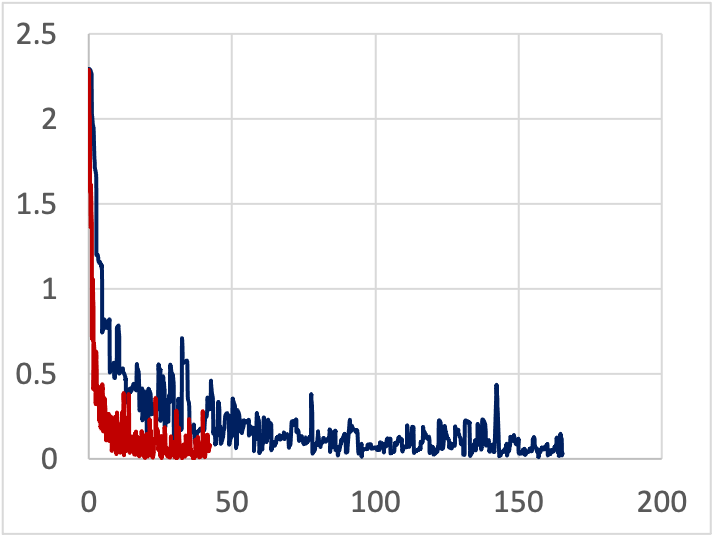
\includegraphics[width=\textwidth]{tape-lstm}
    \caption{LSTM-MNIST}
  \end{subfigure}
  ~
  \begin{subfigure}[t]{.24\textwidth}
    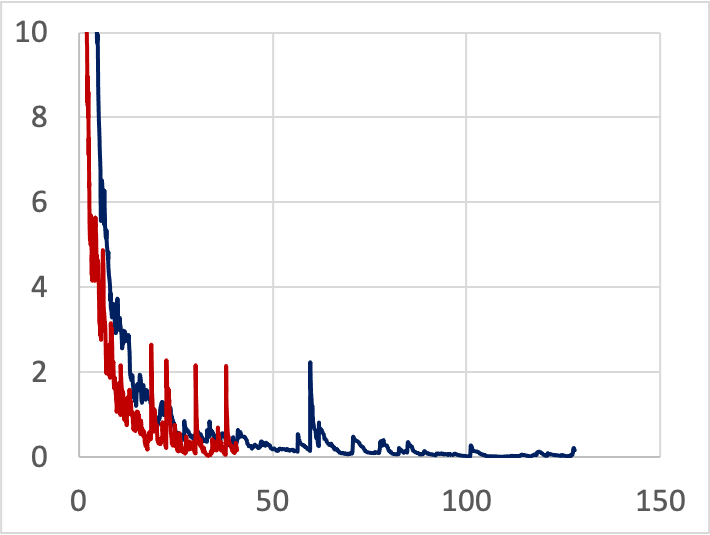
\includegraphics[width=\textwidth]{tape-simple1}
    \caption{SimpleCNN-GradientTape-1}
  \end{subfigure} 
  ~ 
  \begin{subfigure}[t]{.24\textwidth}
    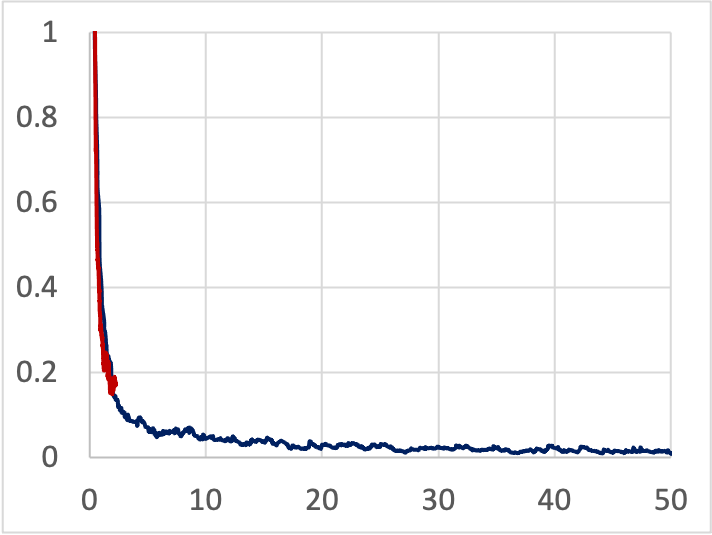
\includegraphics[width=\textwidth]{tape-simple2}
    \caption{SimpleCNN-GradientTape-2}
  \end{subfigure}
  ~
  \begin{subfigure}[t]{.24\textwidth}
    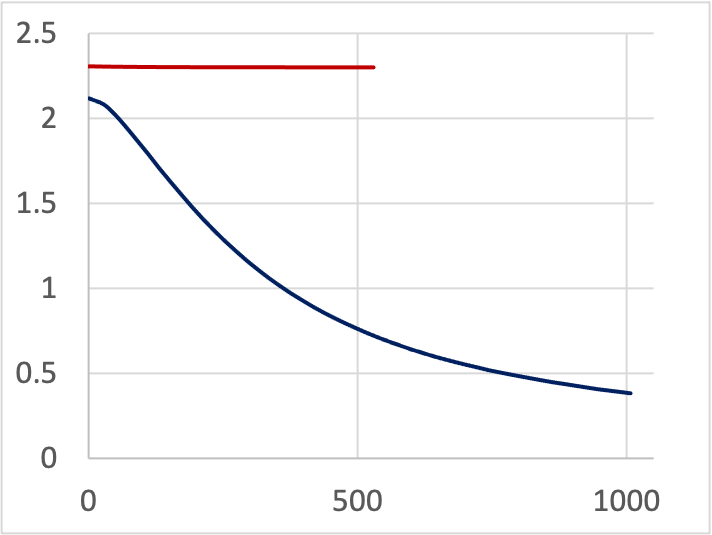
\includegraphics[width=\textwidth]{keras-cifar}
    \caption{VGG-CIFAR10}
  \end{subfigure}

  \begin{subfigure}[t]{.24\textwidth}
    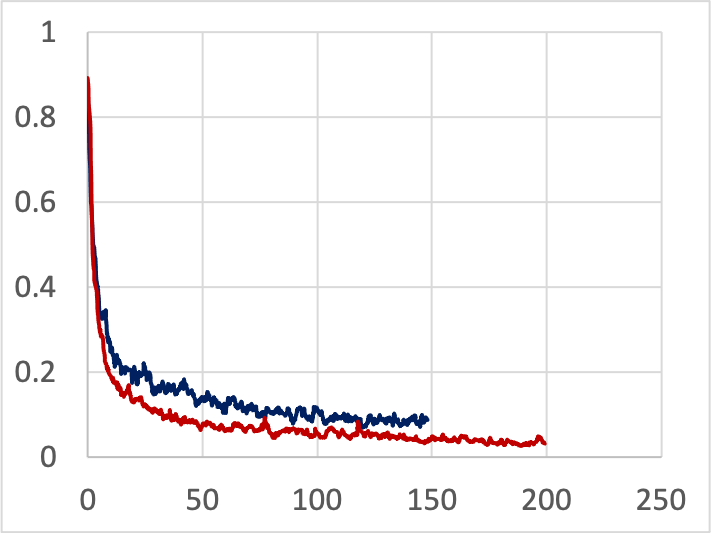
\includegraphics[width=\textwidth]{tf2-03}
    \caption{Play-with-MNIST}
  \end{subfigure}
  ~
  \begin{subfigure}[t]{.24\textwidth}
    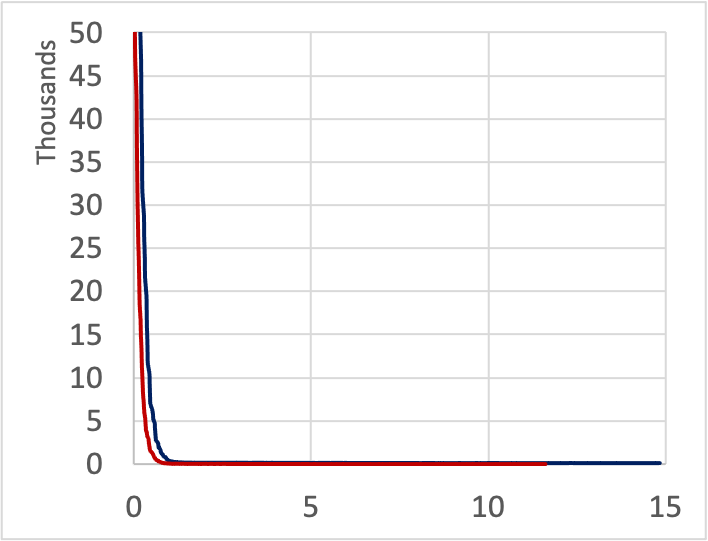
\includegraphics[width=\textwidth]{tf2-04}
    \caption{Linear-Regression}
  \end{subfigure} 
  ~ 
  \begin{subfigure}[t]{.24\textwidth}
    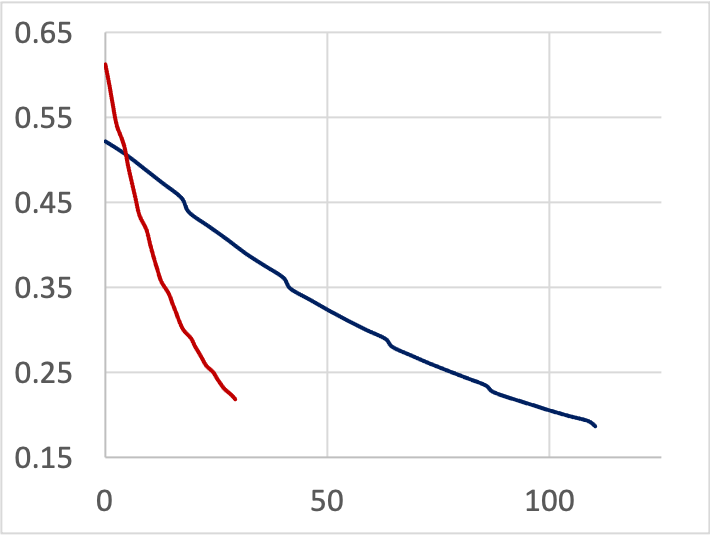
\includegraphics[width=\textwidth]{tf2-05}
    \caption{Fashion-MNIST}
  \end{subfigure}
  ~
  \begin{subfigure}[t]{.24\textwidth}
    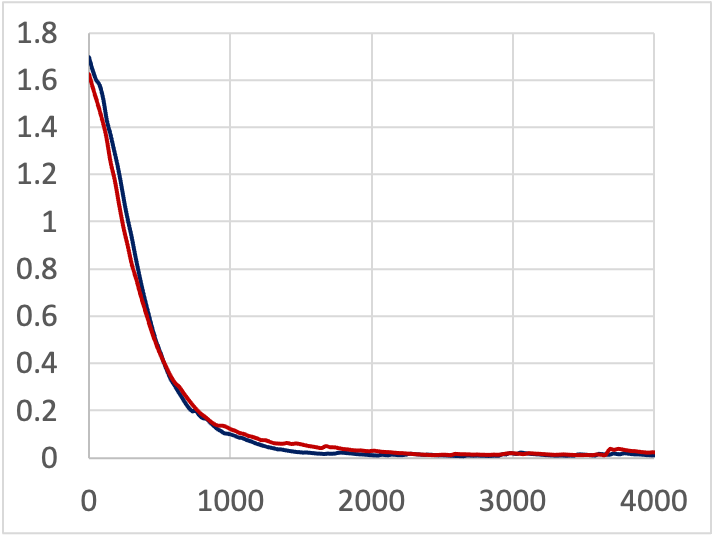
\includegraphics[width=\textwidth]{tf2-06}
    \caption{CIFAR10-VGG16}
  \end{subfigure}

  \begin{subfigure}[t]{.24\textwidth}
    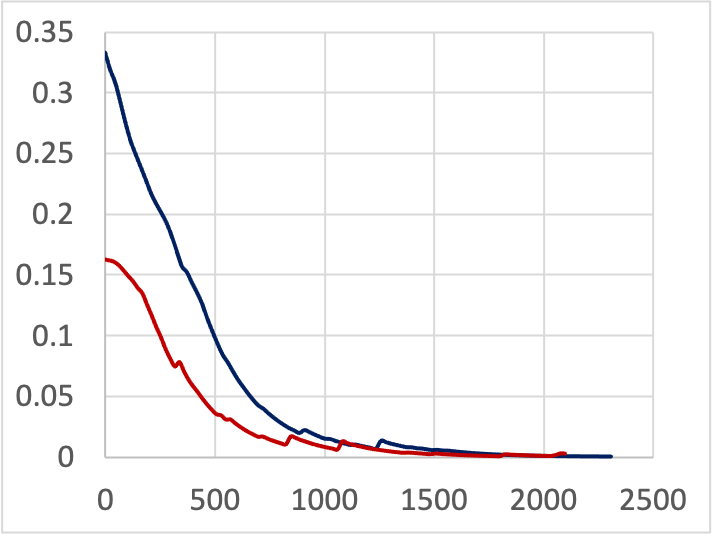
\includegraphics[width=\textwidth]{tf2-07}
    \caption{Inception-network}
  \end{subfigure}
  ~
  \begin{subfigure}[t]{.24\textwidth}
    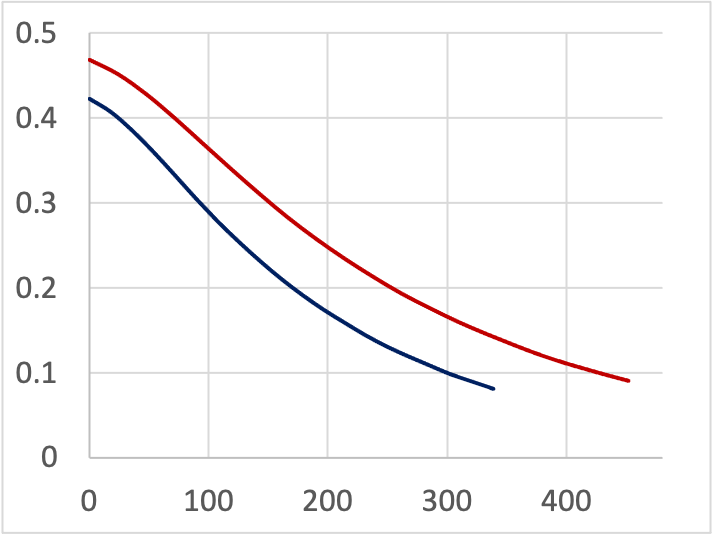
\includegraphics[width=\textwidth]{tf2-09}
    \caption{RNN-Sentiment-Analysis}
  \end{subfigure} 
  ~ 
  \begin{subfigure}[t]{.24\textwidth}
    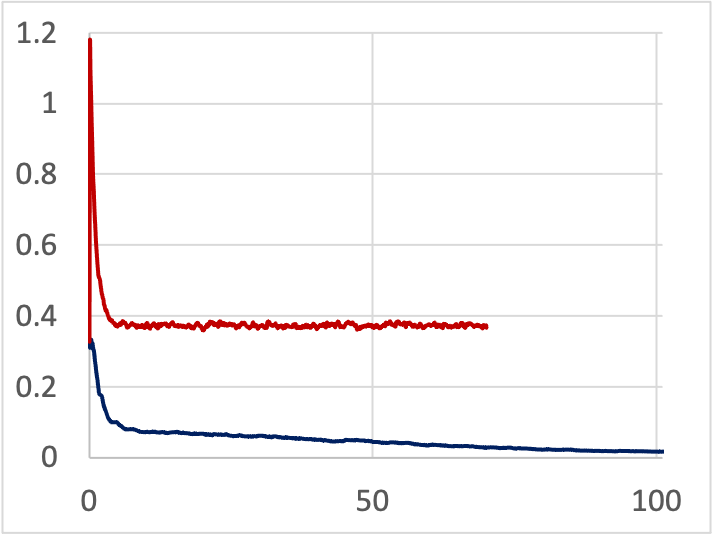
\includegraphics[width=\textwidth]{tf2-10}
    \caption{Stacked-LSTM-ColorBot}
  \end{subfigure}
  ~
  \begin{subfigure}[t]{.24\textwidth}
    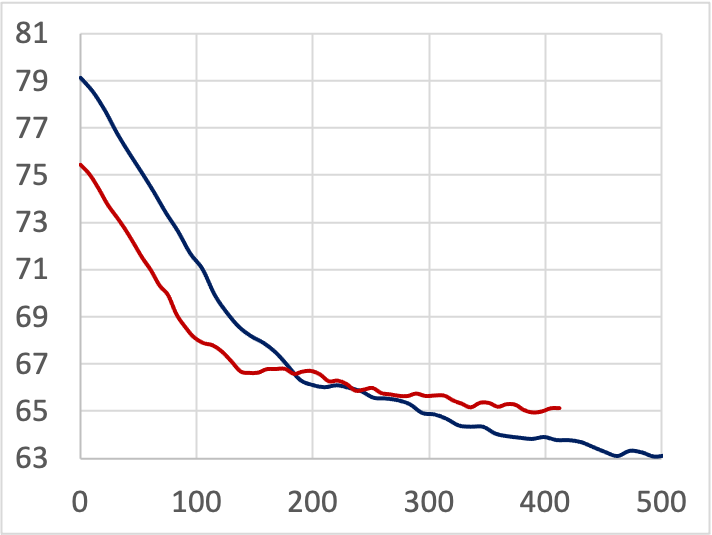
\includegraphics[width=\textwidth]{tf2-11}
    \caption{Auto-Encoder}
  \end{subfigure}

  \begin{subfigure}[t]{.24\textwidth}
    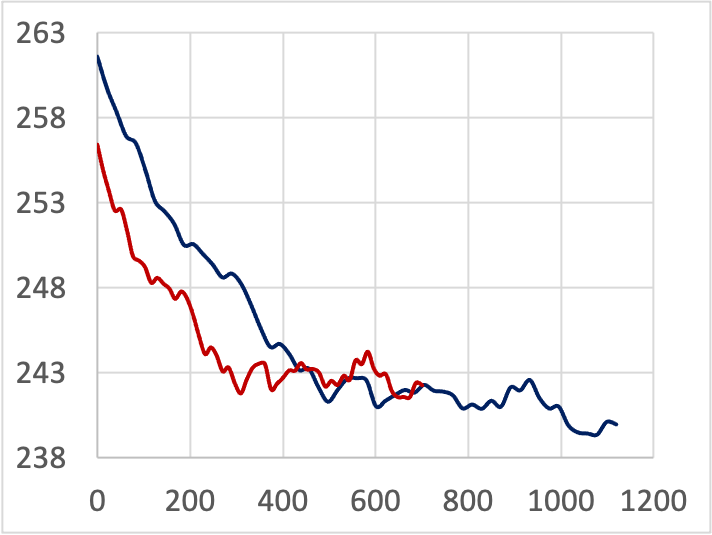
\includegraphics[width=\textwidth]{tf2-12}
    \caption{Variational-Auto-Encoder}
  \end{subfigure}
  ~
  \begin{subfigure}[t]{.24\textwidth}
    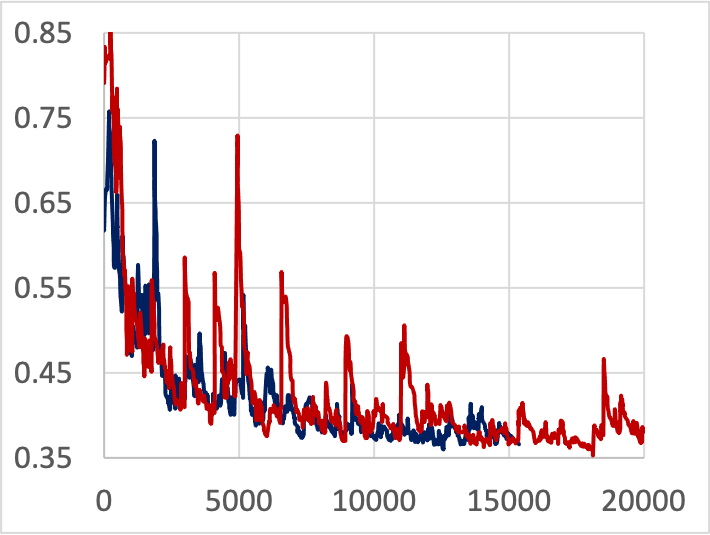
\includegraphics[width=\textwidth]{tf2-13}
    \caption{DCGAN}
  \end{subfigure} 

  \caption{Distributed training experiment result time-loss graphs.}
  \begin{tabular}{r@{: }l r@{: }l}
    X-axis & Time (seconds) & Y-axis & Loss value\\
    Blue line & ORG loss, smoothed & Red line & HVD loss, smoothed\\ 
  \end{tabular}
  \label{fig:eval:train}
\end{figure}

(TODO: include other graphs, too, and make it sane size)

The results of the distributed traininig experiment 
are shown in the figure \ref{fig:eval:train}.
The points in the graphs represent the loss value of the given time;
sky blue points correspond to the \orgbf model training and
orange points coresspond to the \hvdbf model training.
The lines represent the smoothed loss values;
blue lines correspond to the \orgbf model training
and the red lines correspond to the \hvdbf model training.
As shown in the figure, all of the training data show that
the loss value decreases over time, meaning that the training
process is valid.

The distributed training experiment result show that the 8 out of 17 transformed
models show speedup in distributed traininig. The result is rather surprising,
considering that the distributed training itself is successfully executed
without errors. To further investigate the factors that influence the
training speed in the distributed training, 
we performed additional distributed training of some models with
different hyperparameters.

(TODO: include the result of exp with changed lr)

The results show that the training speed difference between single-GPU and
distributed training can differ according to the model hyperparameters
such as the learning rate. The fact that various combinations of hyperparameters
must be considered and experiement to reach optimal training speed is 
well-known in ML community. This problem also applies to distributed training,
where optimial hyperparameters should be re-searched after the training
code is transformed. Our transformation tool do not target to search the 
optimal hyperparameters, although we do implement the guidelines from the
official Horovod documents to scale learning rate and epoch numbers
by number of the GPUs.  

\section{Related Work}\label{sec:related}
We need to survey some related work and describe them here.

\subsection{Distributed DL frameworks}

Many frameworks are developed to support distributed DL training.

TensorFlow provides {\tt tf.distributed.Strategy} API to perform
distributed training across GPUs.
 
Horovod is a multi-framework library for distributed training.

(TODO: find more distributed training frameworks.)

None of these frameworks support automatic transformation from single-GPU
based training to distributed training. 

(TODO: explain that our work is different from using frameworks;
it can automatically transform)

\subsection{Code Transformation}

Code transformation is a technique which source codes are automatically
transformed into another. The techinique is primarily used in compilers,
for optimization process. 

(TODO: find more use case of code transformation)

Note that our approach is not a semantic-preserving code transformation.

(TODO: explain that our's code transformation is different from
compilers and optimization techniques)

Semantic-preserving code transformation for DL model codes should be
further investigated.

\section{Conclusion}\label{sec:conclusion}
We propose the automated approach to transform TensorFlow DL models written in
Python to models training on multiple GPUs.
We defined four common training patterns for TensorFlow DL models and formal
code transformation rules for each pattern to parallelize training via Horovod
APIs.
Also, we developed a code transformation tool that takes a TensorFlow DL model,
identifies its training pattern via static analysis techniques, and rewrites
it for distributed training by applying transformation rules of the identified
training pattern.
The evaluation showed that our approach is practical in that it transforms 15
out of 16 open-source TensorFlow DL models to the same with their handcrafted
distributed training versions.
We also showed that our approach is effective in that the transformed models
train about 2.28 times faster than the original models.
We believe that our tool reduces model engineers' burdens in rewriting models
in accordance with the documentation of distributed training libraries to
parallelize training.

%Our approach classifies TensorFlow DL models into four common training patterns
%we defined, based on their usage of the TensorFlow APIs.
%Then, our approach rewrites models with Horovod APIs by applying transformation
%rules we formally defined for each training pattern.

%By manually inspecting the Horovod document and code examples,
%we defined \textit{training API patterns} for categorizing TensorFlow
%training codes by their API usage, and constructed \textit{transformation rules}
%to distribute the trainig codes of each tranining patterns.

%We implement the transformation in a form of software,
%which includes class hierarchy analysis and pattern analysis to recognize
%the correct transformation rule for the given input model
%and automatically apply the transformation to produce
%the corresponding distributed model as an output.

%We evaluated the correctness of the transformation tool against
%16 open-source DL models, which all but one transformations are
%successful. 

%Evaluating the training performance of the
%transformed model showed us that none or only minimal amounts of
%hyperparameter tuning is required for distributed training speedup. 

%We believe that our transformation tool frees the users from heavy burden of
%rewriting the model code, and allows them to swiftly move from single-GPU-based
%training to distributed training.

%In future works, we aim to search for methods that can fully automate
%the deployments of DL models on distributed systems, including
%automated hyperparameter tunings suited for the distributed system.


% \nocite{*}% Show all bib entries - both cited and uncited; comment this line to view only cited bib entries;


\section*{Author Biography}

\clearpage

\bibliography{ref}%

\bibliography{sn-bibliography}% common bib file

% TODO(all): Add your biography here.
%\begin{biography}{
\includegraphics[width=66pt,height=86pt,draft]{empty}}{\textbf{Author Name.} This is sample author biography text this is sample author biography text this is sample author biography text this is sample author biography text this is sample author biography text this is sample author biography text this is sample author biography text this is sample author biography text this is sample author biography text this is sample author biography text this is sample author biography text this is sample author biography text this is sample author biography text this is sample author biography text this is sample author biography text this is sample author biography text this is sample author biography text this is sample author biography text this is sample author biography text this is sample author biography text this is sample author biography text.}
%\end{biography}

\end{document}
